\documentclass{article}

\usepackage{multicol}
\usepackage{xparse}
\usepackage{graphicx}
\usepackage{breqn}
\usepackage{parskip}
\usepackage{amsmath}
\usepackage{amssymb}
\usepackage{listings}
\usepackage{minted}
\usepackage{csvsimple}
\usepackage{longtable}
\usepackage{soul}
\usepackage{xcolor}
\usepackage{tikz}
\usepackage{circuitikz}
\usepackage{pgfplots}
\usepackage{pgf-umlcd}
\pgfplotsset{width=15cm}
\usepackage{geometry}
  \geometry{
  a4paper,
  left=35mm,
  top=35mm,
 }

\let\ogsection\section
\newcommand{\bigsection}[1]{
  \ogsection{\Large#1}
}

\newenvironment{nodegraph}[0]{
  \begin{tikzpicture}[main/.style = {draw, circle}] 
}{
  \end{tikzpicture}
}
\newcommand{\nodecircle}[2]{
  \node[main] (#1) {#2};
}
\newcommand{\nodecirclerel}[3]{
  \node[main] (#1) {#2} [#3];
}
\newcommand{\nodeline}[2]{
  \draw (#1) -- (#2);
}
\newcommand{\nodearrow}[2]{
  \draw[->] (#1) -- (#2);
}

\setcounter{tocdepth}{3}
\setcounter{secnumdepth}{3}

\begin{document}
  \title{\Huge Appunti Scolastici  Generali Istituto Salvini}
  \author{\Large Matteo Leggio}
  \date{}
  \maketitle

  \section{Prefazione}
  {
    \subsection{Istruzioni di Build}
    I seguenti appunti sono accessibili al pubblico tramite il repository Github `ZenT3600/appunti`. Di seguito si trovano le istruzioni per compilare le sorgenti LaTeX in effettivi documenti PDF condivisibili.

    I pacchetti richiesti per l'operazione sono:
    \begin{itemize}
      \item texlive-most
      \item git
      \item make
    \end{itemize}
    ed un sistema operativo Linux, preferibilmente Arch Linux (il sistema su cui viene compilato solitamente)

    Dopo aver clonato il repository sul proprio sistema con il comando
    \begin{minted}{bash}
      git clone \
      https://github.com/ZenT3600/appunti
    \end{minted}

    Si puo' compilare il codice LaTeX grazie al comando
    \begin{minted}{bash}
      make build clean
    \end{minted}

    \subsection{Note per Scrivere il Sorgente}
    Di seguito alcune note e appunti su come scrivere in maniera corretta e costante il codice sorgente per i medesimi appunti.

    \subsubsection{Colori} % Prefazione - Note per Scrivere il Sorgente
    E' possibile \hl{sottolineare} delle frasi grazie alla sintassi
    \begin{minted}{latex}
      \hl{Testo da sottolineare}
    \end{minted}

    E' inoltre possibile \textcolor{red}{colorare} delle frasi usando la sintassi
    \begin{minted}{latex}
      \textcolor{colore}{Testo da colorare}
    \end{minted}

    \subsubsection{Tipografia} % Prefazione - Note per Scrivere il Sorgente
    La sequente sintassi permette di inserire blocchi di citazioni
    \begin{minted}{latex}
      \begin{quote}
      | Questa e' una citazione
      \end{quote}
    \end{minted}

    La qauale porta ad un risultato come questo
    \begin{quote}
      | Questa e' una citazione
    \end{quote}

    Per ottenere diverse dimensioni di caratteri si puo' usare
    \begin{minted}{latex}
      \small{testo}
      \normalsize{testo}
      \large{testo}
      \Large{testo}
      \LARGE{testo}
      \huge{testo}
    \end{minted}

    Se si vuole scrivere in \textit{italico} o in \textbf{grassetto}, scrivere
    \begin{minted}{latex}
      \textit{italico}
      \textbf{grassetto}
    \end{minted}

    Nel caso in cui si voglia inserire un titolo o sottotitolo la sintassi e'
    \begin{minted}{latex}
      \section{Titolo}
      \subsection{Sottotitolo}
    \end{minted}

    \subsubsection{Note} % Prefazione - Note per Scrivere il Sorgente
    Per generare note a pie' di pagina durante la scrittura del documento si puo' usare
    \begin{minted}{latex}
      Lorem ipsum dolor sit amet
      \footnote{Questo non e' latino!}
    \end{minted}
  }

  \newpage
  \tableofcontents
  \newpage

  \section{Informatica}
  {
    \subsection{Fondamenti di Java}
    \textbf{Java} e' un linguaggio di programmazione \textit{fortemente tipizzato} ed \textit{orientato agli oggetti}. Fortemente tipizzato significa che ogni variabile, o dato, ha un suo tipo \small{(come ad esempio \texttt{int}, \texttt{char}, \texttt{double}, ...)}. Orientato agli oggetti significa che favorisce ed incita la \textbf{Programmazione a Oggetti}, meglio spiegata in un successivo capitolo.

    In Java tutto comincia dal \textbf{main}, il cuore del programma, e tutta la nostra logica deve partire da li'. Il main in Java e' definito come:

    \begin{minted}{java}
      public static void main(String[] args) {
        // Codice
      }
    \end{minted}

    Di seguito sono elencati i vari modi per eseguire determinate operazioni in Java.

    \subsubsection{Variabili} % Informatica - Fondamenti di Java
    Una variabile e' un contenitore per un dato di un determinato tipo a cui viene dato un nome ed un valore. Una variabile si puo' definire nel seguente modo:

    \begin{minted}{java}
      boolean veroOppureFalso = true;
      char carattereSingolo = 'a';      // Singolo apice
      String frase = "ciao mondo"       // Doppio apice
      int intero = 73;
      long interoGigaEnorme = 50438261842;
      float virgola = 87.1;
      double virgolaGigaEnorme = 32829010.32179;
    \end{minted}

    \subsubsection{Array} % Informatica - Fondamenti di Java
    Un array, o vettore, e' un insieme indicizzato e limitato di variabili dello stesso tipo. Indicizzato poiche' ogni variabile e' accessibile grazie alla sua posizione nell'array, con indici che iniziano da 0. Limitato poiche' ogni array ha una grandezza massima ben definita. Un array si puo' definire nel seguente modo:

    \begin{minted}{java}
      // Definiamo un array di interi di dimensione 8
      int[] serieDiFibonacci = new int[8];      // Per gli altri tipi cambia solo la parola 'int'

      // Inseriamo valore nell'array
      serieDiFibonacci[0] = 1;
      serieDiFibonacci[1] = 1;
      serieDiFibonacci[2] = 2;
      serieDiFibonacci[3] = 3;
      serieDiFibonacci[4] = 5;
      serieDiFibonacci[5] = 8;
      serieDiFibonacci[6] = 13;
      serieDiFibonacci[7] = 21;

      // Preleviamo un valore dall'array
      int primoValoreSerie = serieDiFibonacci[0];
    \end{minted}

    \subsubsection{Output} % Informatica - Fondamenti di Java
    Java fornisce due semplici funzioni per mostrare un valore in output, ovvero:

    \begin{minted}{java}
      System.out.println("Scrivi qualcosa e vai a capo");
      System.out.print("Scrivi qualcosa e rimani sulla linea");
    \end{minted}

    \subsubsection{Input} % Informatica - Fondamenti di Java
    Allo stesso modo dell'output, Java fornisce una classe di utilita' per chiedere valori all'utente, ovvero:

    \begin{minted}{java}
      Scanner input = new Scanner(System.in);

      String valoreString = input.nextLine();
      int valoreIntero = input.nextInt();
      float valoreFloat = input.nextFloat();
      // ...
    \end{minted}

    \subsubsection{Condizionali} % Informatica - Fondamenti di Java
    In programmazione i condizionali sono diramazioni del condice in base a una condizione, ovvero una qualsiasi operazione che ritorna un risultato vero, \texttt{true}, o falso, \texttt{false}. Un condizionale, o \texttt{if} per semplicita', e' rappresentabile in Java come:

    \begin{minted}{java}
      int numero = 4;
      if (numero == 4) {        // Nota l'uso del == per la comparazione
        // La condizione e' vera
      } else {
        // La condizione e' falsa
      }
    \end{minted}

    E' inoltre possibile scrivere un \texttt{if} immediatamente dopo un \texttt{else}, creando cosi' una struttura simile a

    \begin{minted}{java}
      if () {
        // codice...
      } else if () {
        // codice...
      } else () {
        // codice...
      }
    \end{minted}

    \subsubsection{Loop} % Informatica - Fondamenti di Java
    Un loop e' una o piu' istruzioni che vengono eseguite ripetutamente. Esistono due tipi di loop in Java:
    
    \begin{itemize}
      \item \textbf{For}, usato per quando si conosce il numero di ripetizioni
      \item \textbf{While}, usato per quando si vuole ripetere finche una condizione non e' vera
    \end{itemize}

    Le sintassi dei due tipi di loop sono le seguenti:

    \begin{minted}{java}
      // For
      for (int i = 0; i < 10; i++) {    // 10 - 0 = 10, percio' il loop viene eseguito 10 volte
        System.out.println(i);
      }

      // While
      int n = 2;
      while (n  < 128) {
        System.out.println(n);
        n = n * 2;
      }
    \end{minted}

    \subsection{Programmazione Procedurale}
    Nella \textbf{programmazione procedurale} un problema, o dominio \small{(ovvero tutte le funzionalità richieste dal cliente)}, é scomposto in \textbf{sottoproblemi} e sono implementati dei \textbf{metodi} che risolvono i sottoproblemi.

    Quindi un metodo non e' altro che \textit{un sottoprogramma, con i suoi input, la sua logica ed i suoi output}. Per assurdo, qualsiasi cosa possiamo sviluppare come metodo, puo' anche essere sviluppata come programma a parte che, opzionalmente, richiede un qualche input.

    \subsubsection{La definizione di un Metodo} % Informatica - Programmazione Procedurale
    Da un punto di vista Java, un metodo e' strutturato nella seguente maniera:

    \begin{quote}
      \texttt{visibilita' ritorno nome(tipo argomento1, tipo argomento2, ...) \{ \}}
    \end{quote}

    Scomponendo le varie parole chiave, possiamo dire che:

    \begin{itemize}
      \item \textbf{Visibilita'} e' la parola chiave che descrive chi puo' usare questo metodo. Le opzioni sono:
      \begin{itemize}
        \item \textit{public}, visibile da tutti
        \item \textit{private}, visibile, nel nostro caso, solo dallo stesso file
        \item \textit{protected}, visibile dallo stesso pacchetto
      \end{itemize}
      \item \textbf{Ritorno} e' il tipo di dato che il metodo dara' in output. Esiste in questo caso il tipo \texttt{void}, che significa nessun ritorno
      \item \textbf{Nome} e' autoesplicativo
      \item \textbf{Tipo Argomento} e' uguale alla definizione di una variabile. Stiamo infatti definendo gli input, o argomenti
    \end{itemize}

    Nella programmazione procedurale bisogna inoltre aggiungere la parola chiave \texttt{static} subito dopo la visibilita'.

    Detto questo, un esempio di effettivo metodo e':

    \begin{minted}{java}
      public static int potenzaDiDue(int numero) {
        return numero * numero;
      }
    \end{minted}

    Per utilizzare il valore che questo metodo restituisce grazie alla parola chiave \texttt{return}, basta scrivere:

    \begin{minted}{java}
      public static void main(String[] args) {
        int seiAllaSeconda = potenzaDiDue(6);   // La variabile contiene ora il risultato del metodo
      }
    \end{minted}

    \subsection{Programmazione a Oggetti}
    Nella \textbf{programmazione a oggetti}, a differenza di quella procedurale, lo stesso problema é invece suddiviso in \textbf{oggetti} fondamentali per il dominio. Ponendo un esempio di un software per gestire una scuola, i vari oggetti potrebbero ad esempio essere variabili di tipo \textit{Alunno}, \textit{Docente}, \textit{Classe} e cosí via.

    \subsubsection{Grafici UML} % Informatica - Programmazione a Oggetti
    I grafici \textbf{UML}, ovvero Unified Modelling Language, fanno parte del linguaggio omonimo, utilizzato per unificare e rendere scientfica la descrizione di varie parti di un programma.

    Vi sono vari tipi di grafici UML, sotto descritti:

    \textbf{Grafici di Classe}
    \begin{quote}
      Un grafico di classe, o \textbf{class diagram} e', al livello piu' semplice, rappresentabile in questa maniera:

      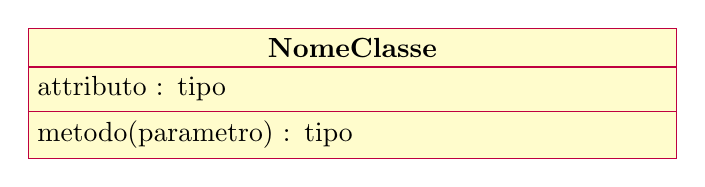
\begin{tikzpicture}
        \begin{class}[text width=8cm]{NomeClasse}{0,0}
          \attribute{attributo : tipo}
          \operation{metodo(parametro) : tipo}
        \end{class}
      \end{tikzpicture}

      Segue un esempio di class diagram che rappresenta un semplice software per gestire un menu' di un ristorante, ignorando per il momento i metodi di ogni classe, che verranno spiegati piu' avanti:

      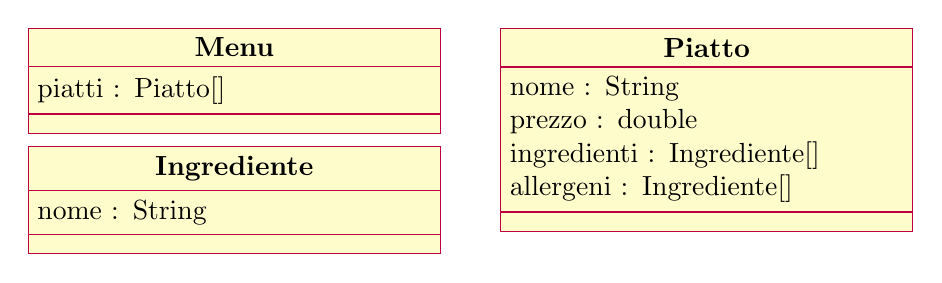
\begin{tikzpicture}
        \begin{class}{Menu}{0,0}
          \attribute{piatti : Piatto[]}
        \end{class}

        \begin{class}{Piatto}{6,0}
          \attribute{nome : String}
          \attribute{prezzo : double}
          \attribute{ingredienti : Ingrediente[]}
          \attribute{allergeni : Ingrediente[]}
        \end{class}

        \begin{class}{Ingrediente}{0,-1.5}
          \attribute{nome : String}
        \end{class}
      \end{tikzpicture}
    \end{quote}
  }

  \pagebreak
  \section{Telecomunicazioni}
  {
    \subsection{Segnali}
    \subsubsection{Segnale Sinusoidale} % Telecomunicazioni - Segnali

    \begin{tikzpicture}
      \begin{axis}[
          axis lines = center,
          xlabel = \(t\),
          ylabel = \(v(t)\),
          ymin = -4,
          ymax = 4,
      ]
        \addplot [
          domain=-10:100,
          color=red,
          samples=200,
        ]{sin(20 * x)};
        \addlegendentry{\(sin(\omega t + \varphi) \times Ap\)}
          \draw [very thick] (axis cs:0,1.5) -- node[above]{$T$} (axis cs:18,1.5);
          \draw [very thin] (axis cs:18,-1) -- (axis cs:18,1.5);

          \draw [very thick] (axis cs:-5,0) -- node[left, yshift=.5cm]{$Ap$} (axis cs:-5,1);
          \draw [very thin] (axis cs:-5,0) -- (axis cs:0,0);
          \draw [very thin] (axis cs:-5,1) -- (axis cs:0,1);
      \end{axis}
    \end{tikzpicture}

    Valori fondamentali:

    $$ \omega ^{(pulsazione)} = \frac{2\pi}{T} = 2\pi f $$
    $$ f ^{(frequenza)} = \frac{1}{T} $$
    $$ \varphi ^{(fase)} = v(0) $$
    $$ Ap ^{(ampiezza)} $$
    $$ T ^{(periodo)} $$
    $$ \lambda ^{(lunghezza d'onda)} = \frac{c ^{(velocita' della luce)}}{f} $$

    \subsubsection{Segnale Sinusoidale nei Numeri Complessi} % Telecomunicazioni - Segnali
    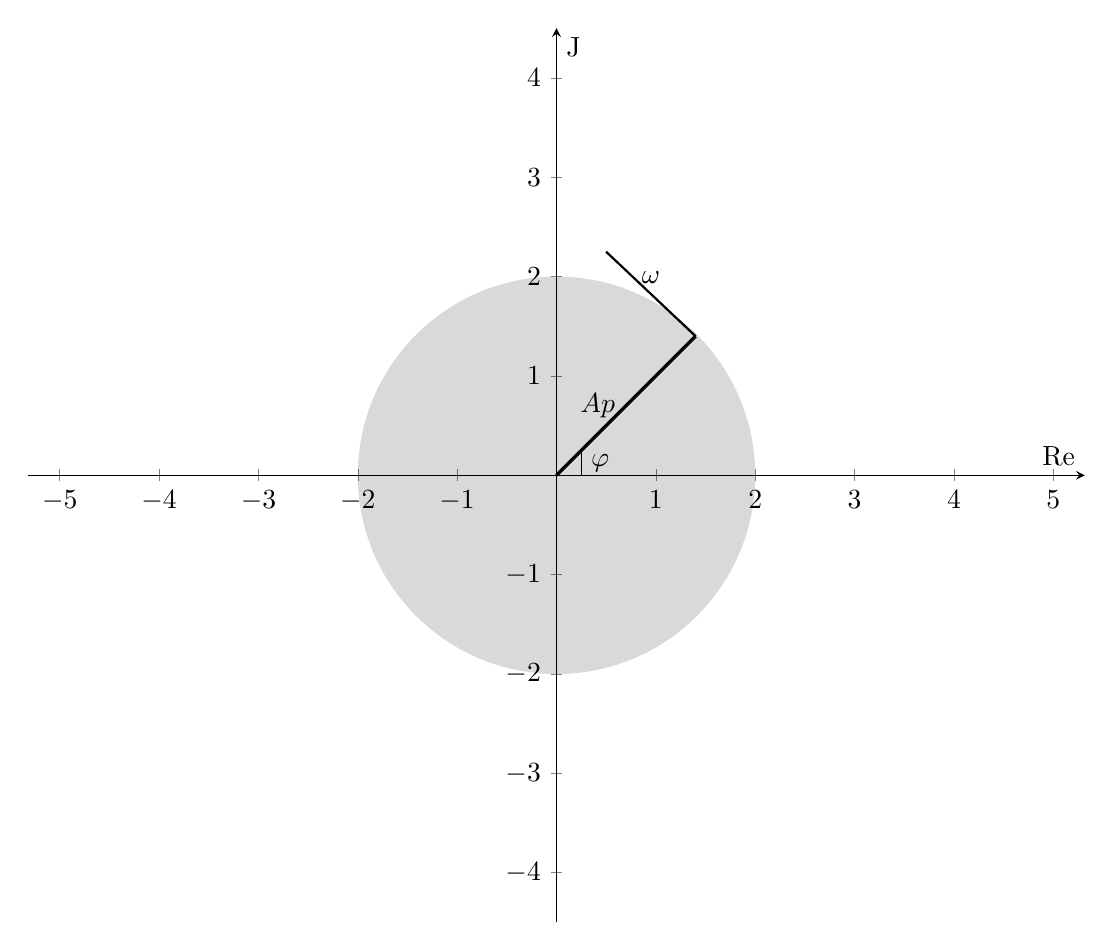
\begin{tikzpicture}
  \begin{axis}[
      xmin=-4.5,
      xmax=4.5,
      ymin=-4.5,
      ymax=4.5,
      axis equal,
      axis lines=middle,
      xlabel=Re,
      ylabel=J,
      disabledatascaling
  ]
      \fill [opacity=0.15] (0,0) circle [radius=2];
      \draw [very thick] (axis cs:0,0) -- node [left]{$Ap$} (axis cs:1.4,1.4);
      \draw [thick] (axis cs:1.4,1.4) -- node [above]{$\omega$} (axis cs:0.5,2.25);
      \draw [] (axis cs:0.25,0) -- node [right]{$\varphi$} (axis cs:0.25,0.25);
  \end{axis}
    \end{tikzpicture}

    \break

    \subsection{Circuiti}
    \subsubsection{Circuiti Resistivi} % Telecomunicazioni - Circuiti
    Un circuito e' detto puramente resistivo quando \textbf{continene solamente resistenze}. Lo schema generico e' come segue:

    \begin{circuitikz}
      \draw
      (0,0) to[sinusoidal voltage source, l=V] (0,4) -- (4,4)
      to[R, l=R] (4,0) -- (0,0)
      ;
    \end{circuitikz}

    Per calcolare la I, possiamo usare la relazione

    $$ V = I \times R $$

    Ed eseguire percio' un prodotto scalare pari a:

    $$ I = \frac{V}{R} $$

    \subsubsection{Circuiti Capacitivi} % Telecomunicazioni - Circuiti
    Un circuito e' detto puramente capacitivo quando \textbf{continene solamente condensatori}. Lo schema generico e' come segue:

    \begin{circuitikz}
      \draw
      (0,0) to[sinusoidal voltage source, l=V] (0,4) -- (4,4)
      to[C, l=C] (4,0) -- (0,0)
      ;
    \end{circuitikz}
    
    Questo circuito contiene \textbf{reattanza capacitiva}, ovvero l'ostacolo che il condensatore pone al passaggio di corrente, con simbolo $ X_C $ [$\Omega$] e calcolabile come

    $$ X_C = \frac{1}{\omega \times C} $$

    Dove

    $$ \omega = 2\pi \times f $$

    Si puo' quindi, secondo la legge di Ohm, scrivere che

    $$ V = -j X_C \times I $$

    Si osserva percio' che la corrente $ I $ e' sfasata in \textbf{ritardo} di 90 gradi rispetto alla $ V $.

    \subsubsection{Circuiti Induttivi} % Telecomunicazioni - Circuiti
    Un circuito e' detto puramente induttivo quando \textbf{continene solamente induttori}. Lo schema generico e' come segue:

    \begin{circuitikz}
      \draw
      (0,0) to[sinusoidal voltage source, l=V] (0,4) -- (4,4)
      to[L, l=L] (4,0) -- (0,0)
      ;
    \end{circuitikz}
    
    Questo circuito contiene \textbf{reattanza induttiva}, ovvero l'ostacolo che l'induttore pone al passaggio di corrente, con simbolo $ X_L $ [$\Omega$] e calcolabile come

    $$ X_L = \omega \times L $$

    Dove

    $$ \omega = 2\pi \times f $$

    Si puo' quindi, secondo la legge di Ohm, scrivere che

    $$ V = j X_L \times I $$

    E percio' dire che la corrente $ I $ e' sfasata in \textbf{anticipo} di 90 gradi rispetto alla $ V $.

    \subsubsection{Circuiti RC} % Telecomunicazioni - Circuiti
    Un circuito e' detto RC quando \textbf{continene sia resistenze che condensatori}. Lo schema generico e' come segue:

    \begin{circuitikz}
      \draw
      (0,0) to[sinusoidal voltage source, l=V] (0,4)
      to[R, l=R] (4,4)
      to[C, l=C] (4,0) -- (0,0)
      ;
    \end{circuitikz}

    Per risolvere questo circuito bisogna anzitutto calcolare $ X_C $ come in un circuito capacitivo e, successivamente, utilizzare il teorema di pitagora per ottenere l'impedenza $ Z $ e la sua relativa fase $ \varphi $

    $$ Z = \sqrt{R^2 + X_C^2} $$

    $$ \varphi = arctg(\frac{X_C}{R}) $$
 

    \subsubsection{Circuiti RL} % Telecomunicazioni - Circuiti
    Un circuito e' detto RL quando \textbf{continene sia resistenze che induttori}. Lo schema generico e' come segue:

    \begin{circuitikz}
      \draw
      (0,0) to[sinusoidal voltage source, l=V] (0,4)
      to[R, l=R] (4,4)
      to[L, l=L] (4,0) -- (0,0)
      ;
    \end{circuitikz}

    Per risolvere questo circuito bisogna anzitutto calcolare $ X_L $ come in un circuito induttivo o e, successivamente, utilizzare il teorema di pitagora per ottenere l'impedenza $ Z $ e la sua relativa fase $ \varphi $

    $$ Z = \sqrt{R^2 + X_L^2} $$

    $$ \varphi = arctg(\frac{X_L}{R}) $$
 
    \subsubsection{Circuiti RLC} % Telecomunicazioni - Circuiti
    Un circuito e' detto RLC quando \textbf{continene resistenze, induttori e condensatori}. Lo schema generico e' come segue:

    \begin{circuitikz}
      \draw
      (0,0) to[sinusoidal voltage source, l=V] (0,4)
      to[R, l=R] (4,4)
      to[L, l=L] (4,0)
      to[C, l=C] (0,0)
      ;
    \end{circuitikz}

    Per risolvere questo circuito bisogna anzitutto calcolare $ X_C $ ed $ X_L $ come in un circuito capacitivo ed uno induttotivo e, successivamente, utilizzare il teorema di pitagora per ottenere l'impedenza $ Z $ e la sua relativa fase $ \varphi $

    $$ Z = \sqrt{R^2 + (X_L^2 - X_C^2)} $$

    $$ \varphi = arctg(\frac{X_L - X_C}{R}) $$
  }

  \pagebreak
  \section{Sistemi e Reti}
  {
    \subsection{Calcoli su Indirizzi IP}
    A partire da un'indirizzo IP con una maschera di sottorete, quale ad esempio \textit{130.1.10.32/20} e' possibile ottenere ulteriori informazioni sulla rete, quali l'indirizzo di rete e l'indirizzo di broadast, a partire dai seguenti calcoli:

    $$ IP_{10} = 130.1.10.32 $$ 
    $$ IP_{2} = 10000010.00000001.00001010.00100000 $$
    $$ SM_{10} = 20 $$
    $$ SM_{2} = 11111111.11111111.11110000.00000000 $$
    $$ IR_{2} = IP_{2} \cdot SM_{2} = 10000010.00000001.00000000.00000000 $$
    $$ IB_{2} = IP_{2} + CM_{1}(SM_{2}) = 10000010.00000001.00001111.11111111 $$

    Il \textbf{subnetting} e' una tecnica che permette di dividere una rete in sottoreti utilizzando la parte host di un indirizzo IP. Esistono due metodi per eseguire il subnetting, in base alla maschera di rete usata: Maschera Fissa e Maschera Mobile.

    \textbf{Maschera Fissa}
    \begin{quote}
      Per capire quanti bit bisogna rubare alla parte host dell'IP, bisogna trovare il multiplo di 2 minimo necessario per contenere le sottoreti richieste. Per esempio se c'e' bisogno di 4 sottoreti, si ruberanno 2 bit alla parte host, poiche' $ 2^2 = 4 $ La subnet mask sara' poi $ 24 + 2 = 26 $. Si otterranno percio' le seguenti sottoreti:

      \begin{tabular}{ |c|c| }
        \hline
        Rete & Binario \\
        \hline
        192.168.5.0/26 & 11000000.10101000.00000101.\textbf{00}000000 \\
        192.168.5.64/26 & 11000000.10101000.00000101.\textbf{01}000000 \\
        192.168.5.128/26 & 11000000.10101000.00000101.\textbf{10}000000 \\
        192.168.5.192/26 & 11000000.10101000.00000101.\textbf{11}000000 \\
        \hline
      \end{tabular}
    \end{quote}

    \textbf{Maschera Mobile}
    \begin{quote}
      Quella della maschera mobile e' una tecnica sviluppata per risparmiare nella creazione di sottoreti. Per capire quanti bit bisogna usare, si trova la $ x $ per $ 2^x \geqslant h_{richiesti} $. Trovata la $ x $, la maschera della sottorete sara' $ 32 - x $ e gli host inizieranno dall'ottetto finale della rete precedente sommato a $ 1 $ e finiranno con l'ottetto final della rete corrente sommato $ 2^x $ e sottratto $ 1 $. Dopodiche', si passa alla prossima sottorete e si ripete. Il risultato ottenuto e' una serie di rete con maschera di rete diversa.

      Esempio:

      \begin{tabular}{ |c|c|c| }
        \hline
        Rete & Numero Sottoreti & Host Richiesti \\
        \hline
        193.80.1.0/24 & 4 & 40, 30, 10, 6 \\
        \hline
      \end{tabular}

      \begin{tabular}{ |c|c|c|c| }
        \hline
        Rete & Mask & Da & a \\
        \hline
        A & /26 & 193.80.1.1 & 193.80.1.63 \\
        B & /27 & 193.80.1.64 & 193.80.1.95 \\
        C & /28 & 193.80.1.96 & 193.80.1.111 \\
        D & /29 & 193.80.1.112 & 193.80.1.119 \\
        \hline
      \end{tabular}
    \end{quote}

    \break

    \subsection{Grafi}
    Un grafo e' un tipo di struttura matematica consistente di \textbf{nodi uniti da archi}, formando una specie di ragnatela. I grafi possono essere pesati o meno a seconda se il traversare un arco ha un costo maggiore rispetto ad un altro. I grafi possono inoltre essere orientati se un qualsiasi arco puo' essere percorso in una direzione, ma non all'incontrario.

    Un esempio di grafo e':

    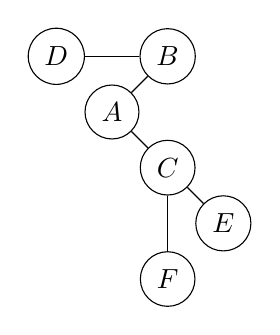
\begin{tikzpicture}[main/.style = {draw, circle}] 
      \node[main] (1) {$A$};
      \node[main] (2) [above right of=1] {$B$};
      \node[main] (3) [below right of=1] {$C$};
      \node[main] (4) [above left of=1] {$D$};
      \node[main] (5) [below right of=3] {$E$};
      \node[main] (6) [below left of=5] {$F$};

      \draw[-] (1) -- (2);
      \draw[-] (2) -- (4);
      \draw[-] (1) -- (3);
      \draw[-] (3) -- (5);
      \draw[-] (3) -- (6);
    \end{tikzpicture}

    Dove i cerchi contenenti lettere rappresentano i nodi e le linee rappresentano gli archi.
    
    \subsubsection{Matrice di Adiacenza} % Sistemi e Reti - Grafi
    Per rappresentare un grafo in maniera numerica si puo' utilizzare una matrice di adiacenza, ovvero una tabella simile alla seguente.

    \begin{tabular}{ |c|c|c|c|c|c|c| }
      \hline
        & A & B & C & D & E & F \\
      A & 0 & 1 & 0 & 1 & 0 & 0 \\
      B & 1 & 0 & 0 & 1 & 0 & 0 \\
      C & 1 & 0 & 0 & 0 & 1 & 1 \\
      D & 0 & 1 & 0 & 0 & 0 & 0 \\
      E & 0 & 0 & 1 & 0 & 0 & 0 \\
      F & 0 & 0 & 1 & 0 & 0 & 0 \\
      \hline
    \end{tabular}

    Dove 0 rappresenta una connessione inesistente, mentre 1 rappresenta una connessione. Nel caso di grafi pesati si usa, al posto del numero 1, il peso del relativo ramo.

    \subsubsection{Visita} % Sistemi e Reti - Grafi
    Per visita di un grafo si intende \textbf{l'operazione di trovare gli archi minimi necessari a connettere l'intero grafo}. Per svolgere questa operazione esistono vari algoritmi, come i seguenti:

    \textbf{Kruskal}
    \begin{quote}
      L'algoritmo di Kruskal afferma che, per visitare un grafo, bisogna mettere in ordine crescente i pesi del grafo interessato ed evidenziare gli archi in ordine, purche l'arco da evidenziare non chiuda una forma geometrica con gli altri archi.
    
    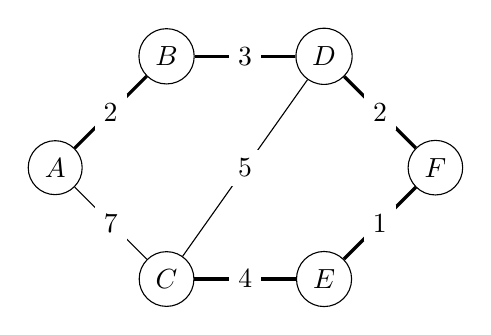
\begin{tikzpicture}[node distance=20mm, main/.style = {draw, circle}] 
      \node[main] (1) {$A$};
      \node[main] (2) [above right of=1] {$B$};
      \node[main] (3) [below right of=1] {$C$};
      \node[main] (4) [right of=2] {$D$};
      \node[main] (5) [right of=3] {$E$};
      \node[main] (6) [below right of=4] {$F$};

      \draw[very thick] (1) -- (2) node[midway, fill=white] {2};
      \draw[-] (1) -- (3) node[midway, fill=white] {7};
      \draw[very thick] (2) -- (4) node[midway, fill=white] {3};
      \draw[very thick] (3) -- (5) node[midway, fill=white] {4};
      \draw[very thick] (5) -- (6) node[midway, fill=white] {1};
      \draw[very thick] (4) -- (6) node[midway, fill=white] {2};
      \draw[-] (3) -- (4) node[midway, fill=white] {5};
    \end{tikzpicture}

    \end{quote}
  }

  \pagebreak
  \section{TPSIT}
  {
    \subsection{Algoritmi di Scheduling}
    Gli algoritmi di scheduling sono algoritmi utilizzati dallo \textbf{scheduler di processi} all'interno di un sistema che servono a ridurre al minimo i tempi di attesa dei vari processi.

    Di seguito sono gli algoritmi principali, assieme ad un grafico rappresentante quegli stessi algoritmi.

    \subsubsection{First come, First served} % TPSIT - Algoritmi di Scheduling
    Questo algroritmo, detto anche FCFS, e' basato su di una struttura dati detta \textbf{Coda FIFO}, immaginabile come una coda ad un supermercato, dove il primo che entra e' il primo che esce. Questo algoritmo, percio' \textbf{posiziona i processi in coda in base al tempo di arrivo}.

    \subsubsection{Shortest Job First} % TPSIT - Algoritmi di Scheduling
    Questo algoritmo, detto anche SJF, si fonda sull'idea che il processo piu' corto debba essere eseguito per primo. Questo algoritmo puo' essere interpretato in due modi:

    \textbf{Senza Prelazione}
    \begin{quote}
      Questo algoritmo \textbf{posiziona i processi in coda in base al tempo di arrivo ed al tempo di durata}, tuttavia \textbf{non puo' fermare un processo in esecuzione}.
    \end{quote}

    \textbf{Con Prelazione}
    \begin{quote}
      Questo algoritmo si comporta come la sua controparte, con la differenza che \textbf{ha la capacita' di fermare un processo in esecuzione, rimettendolo in coda, qualora arrivi un processo piu' corto}.
    \end{quote}

    \subsubsection{Round Robin} % TPSIT - Algoritmi di Scheduling
    Questp algoritmo si comporta in maniera simile all'FCFS, richiedendo pero' un parametro di tempo detto \textbf{quanto}. L'algoritmo \textbf{ferma e rimette in coda un il processo in esecuzione una volta che esso e' rimasto in esecuzione per un tempo pari al quanto}. 

    \subsubsection{Esempio} % TPSIT - Algoritmi di Scheduling
    Volendo dare un esempio di questi algoritmi, basandoci sui seguenti processi, essi si comportano cosi':

    \begin{tabular}{ |c|c|c| }
      \hline
      ID Processo & Tempo di Durata & Tempo di Arrivo \\
      \hline
      1 & 10 & 1 \\
      2 & 5 & 2 \\
      3 & 7 & 3 \\
      4 & 2 & 4 \\
      \hline
    \end{tabular}

    \newcommand{\ProcessGraph}[4]{
      \addplot [
        domain=#2:#3,
        color=#4,
      ]{#1};
    }

    \begin{tikzpicture}
      \begin{axis}[
          axis lines = middle,
          ylabel = \(process\),
          xlabel = \(t\),
          ymin = 0,
          ymax = 10,
          legend entries = {
            First come First served,
            Shortest Job First Senza Prelazione,
            Shortest Job First Con Prelazione,
            Round Robin Con Quanto da 4,
          },
      ]
        \addlegendimage{no markers,red};
        \addlegendimage{no markers,blue};
        \addlegendimage{no markers,teal};
        \addlegendimage{no markers,orange};

        \ProcessGraph{1}{0}{10}{red}
        \ProcessGraph{2}{10}{15}{red}
        \ProcessGraph{3}{15}{22}{red}
        \ProcessGraph{4}{22}{24}{red}

        \ProcessGraph{1.1}{0}{10}{blue}
        \ProcessGraph{4.1}{10}{12}{blue}
        \ProcessGraph{2.1}{12}{17}{blue}
        \ProcessGraph{3.1}{17}{24}{blue}

        \ProcessGraph{1.2}{0}{2}{teal}
        \ProcessGraph{2.2}{2}{4}{teal}
        \ProcessGraph{4.2}{4}{6}{teal}
        \ProcessGraph{2.2}{6}{9}{teal}
        \ProcessGraph{3.2}{9}{16}{teal}
        \ProcessGraph{1.2}{16}{24}{teal}

        \ProcessGraph{1.3}{0}{4}{orange}
        \ProcessGraph{2.3}{4}{8}{orange}
        \ProcessGraph{3.3}{8}{12}{orange}
        \ProcessGraph{4.3}{12}{14}{orange}
        \ProcessGraph{1.3}{14}{18}{orange}
        \ProcessGraph{2.3}{18}{19}{orange}
        \ProcessGraph{3.3}{19}{22}{orange}
        \ProcessGraph{1.3}{22}{24}{orange}
      \end{axis}
    \end{tikzpicture}

  \subsection{Gestione della Memoria}
  La gestione della memoria deve minimizzare l'\textit{overhead}, ovvero i tempi di attesa, e massimizzare l'utilizzo della memoria

  \subsubsection{Concetti Base} % TPSIT - Gestione della Memoria
  \begin{itemize}
    \item \textbf{Allocazione e Deallocazione}: inserire e togliere dalla memoria
    \item \textbf{Protezione e Condivisione}: alcuni pezzi della memoria vanno condivisi per poter essere usati da tutti i processi, altri vanno protetti perché contengono dati sensibili
    \item \textbf{Swapping}: il processo per cui si alloca una parte di memoria RAM in un file sul disco, per quando la RAM é completamente piena e non c'é altro luogo dove scrivere i dati
    \item \textbf{Rilocazione Statica e Dinamica}: nella statica la memoria non é swappabile, nella dinamica si
    \item \textbf{Paginazione}: la memoria é divisa in pagine, i processi in frame. ogni frame rientra in una pagina e punta alla pagina successiva: questo permette di fingere un senso di sequenzialità della memoria
  \end{itemize}

  \subsubsection{Partizionamento} % TPSIT - Gestione della Memoria
  la memoria é organizzata in \textit{partizioni} ovvero spazi di memoria. ci sono vari tipi di partizionamento:
  \begin{itemize}
    \item \textbf{Fisso}: tutte le partizioni sono di uguale dimensione. questo lascia spazio vuoto all'interno delle partizioni (frammentazione interna) visto che puó esserci un solo processo per partizione e non é detto sia grande quanto essa 
    \item \textbf{Dinamico}: le partizioni sono di dimensione variabile, grandi quanto richiesto dal processo. risolve la frammentazione interna ma introduce la frammentazione esterna (quando un processo viene deallocato rimane uno spazio vuoto che non é detto si possa riempire).
  \end{itemize}
  
  per risolvere la frammentazione esterna si usano vari algoritmi di gestione della memoria:
  \begin{itemize}
    \item \textbf{Best-Fit}: i processi si allocano nello spazio più piccolo disponibile (lento, bisogna trovare tutti i buchi)
    \item \textbf{First-Fit}: i processi si allocano nel primo spazio che puó contenerlo a partire dall'inizio della memoria
    \item \textbf{Next-Fit}: come il first fit ma si parte dall'ultimo processo allocato invece che dall'inizio della memoria
  \end{itemize}

  \subsection{Tipi di Processo}
  \subsubsection{Processi Pesanti e Leggeri} % TPSIT - Tipi di Processo
  I processi possono essere divisi a seconda dell'impatto e l'utilizzo delle risorse. Secondo questa divisione, esistono due tipi di processi: Pesanti (Heavy) e Leggeri (Light).

  I \textbf{processi pesanti ottengono risorse} e sono lanciati \textbf{dal sistema}. Essi sono visualizzabili come i vari programmi che il computer esegue.

  I \textbf{processi leggeri sono eseguiti all'interno di un processo pesante}. Essi sono visualizzabili come \textbf{thread} di un programma esistente.

  Per porre un esempio, all'interno di una cucina di alta pasticceria un processo pesante potrebbe essere pasticciere capo, che decide di cucinare una torta, mentre i processi leggeri potrebbe essere rappresentati dai cuochi responsabili delle varie parti della torta (la crema, la panna montata, gli strati...). Ciascuno cuoco \textbf{deve condividere le stesse risorse} (i fornelli, l'abbattitore, il frullatore, gli ingredienti...)

  \subsubsection{Processi Sequenziali e Paralleli} % TPSIT - Tipi di Processo
  I processi possono anche essere divisi a seconda della loro gestione del tempo di esecuzione. Secondo questa divisione, esistono due tipi di processi: Sequenziali e Paralleli.

  I \textbf{processi sequenziali eseguono le operazioni una dopo l'altra}. Cio' significa che due processi sequenziali dovranno fare a turno per andare in esecuzione.

  I \textbf{processi paralleli vengono eseguiti in contemporanea con altri processi}. Questo significa che due processi paralleli possono eseguire le loro operazioni allo stesso tempo. Sia chiaro che, affinche' i processi possano effetitivamente essere paralleli, e' richiesta una CPU con piu' core.
 }

  \pagebreak
  \section{Letteratura}
  {
    \subsection{Eta' del Barocco}
    \subsubsection{La lirica in Italia} % Letteratura - Eta' del Barocco
    \textbf{Giovan Battista Marino} soddisfa le esigenze di rinnovamento letterario del barocco grazie alla sua poesi innovatrice. Il suo stile presenta principalmente:
    
    \begin{itemize}
      \item Un modo artificioso di imporsi sull'attenzione dei lettori
      \item Un uso sistematico di metafore e concetti
      \item Un controllo della retorica e della musicalita' del verso
      \item Un accostamento di immagini e concetti reali solitamente considerati distanti fra loro \small{(Ad esempio il verso mariniano "\textit{onde dorate, e l'onde eran capelli}")}
    \end{itemize}

    \textbf{Gabriello Chiabrera} da Savona, invece che sul gioco metaforico, concentra la sua ricerca sull'aspetto musicale della poesia. Era considerato dai contemporanei un difensore della classicita', mentre e' adesso considerato un innovatore proprio per questa sperimentazione stilistica.

    \subsubsection{La lirica in Spagna e in Inghilterra} % Letteratura - Eta' del Barocco
    \textbf{Luis de Gongora} e \textbf{Francisco de Quevedo} sono l'esempio massimo del concettismo Barocco in Spagna. Le loro opere \textbf{influenzarono la poesia fino al tardo ottocento}.

    \textbf{John Donne}, facente parte dei contamporanei "poeti metafisici", sviluppa in Inghilterra il linguaggio metaforico e immaginifico. I componimenti di questo movimento era pieni di accostamenti tra sentimento e ragione ed affrontavano \textbf{temi dell'esistenza umana} come l'amore e la morte. Il loro stile \textbf{viene ripreso dalla poesia inglese del Novecento}.
    
    \subsubsection{La decadenza del poema epico} % Letteratura - Eta' del Barocco
    Nonostante i vari testi epici di \textbf{Torquato Tasso} il modello epico, gia criticato da Ariosto, continua il suo declino. Durante il periodo barocco, esso subisce un \textbf{rovesciamento dei criteri e dei valori del genere stesso} per via di due poemi volutamente anormali:
    
    \begin{itemize}
      \item \textit{La secchia rapita} di Alessandro Tassoni
      \begin{itemize}
        \item Narra di un'immaginaria guerra tra Modena e Bologna per il possesso di una secchia di legno
        \item Usa il modello epico dell'\textit{Iliade} di Omero
        \item Racconta un contenuto basso con una forma alta, ottenendo un effetto comico
      \end{itemize}
      \item \textit{Adone} di Giovan Battista Marino
      \begin{itemize}
        \item Consistente in un'infita serie di descrizioni, digressioni e racconti secondari lievemente collegate
        \item Il poeta descrive le esperienze sensuali ed erotiche come le uniche capaci di rivelare il senso dell'esistenza all'uomo
        \item Realizza una piena \textit{estinzione del racconto}
      \end{itemize}
    \end{itemize}

    \subsubsection{La propaganda religiosa} % Letteratura - Eta' del Barocco
    La chiesa viene spinta ad usare forme del marinismo nelle sue prediche per attrare le masse. I massimi esponenti di questo e' \textbf{Emanuele Orchi} e \textbf{Daniello Bartoli}, quest'ultimo principalmente con \textit{Storia della Compagnia di Gesu'}.

    \subsubsection{La prosa scientifica} % Letteratura - Eta' del Barocco
    \textbf{Galileo Galilei} adotta il modello del dialogo platonico a due o piu' voci, in quanto lo crede utile ed innovativo per esporre tesi contrastanti.

    Un'esempio di questo si ha nel \textit{Dialogo sopra i due massimi sistemi del mondo}, dove un sostenitore del sistema copernicano ed uno del sistema tolemaico davanti ad una persona non colta in quanto a scienza, la quale trova pian piano sempre piu' ragionevole il sistema copernicano. Galileo dona alle proprie voci vere e proprie sagome con spessore umano, incoraggiado il lettore a prendere posizione, e scrive in volgare, per assicurarsi una diffusione massima.

    All'esempio di Galileo si rifaranno successivamente autori come \textbf{Lorenzo Magalotti} e \textbf{Francesco Redi}.


    \subsubsection{Il romanzo in Italia} % Letteratura - Eta' del Barocco
    Durante il Seicento, in Italia nasce il romanzo e divene famoso per la sua capacita' di conquistare il pubblico e i suoi temi attuali. Il romanzo meglio riuscito del tempo si ha con il \textit{Calloandro fedele} di \textbf{Giovanni Ambrogio Marini}

    \subsubsection{La novella in Italia} % Letteratura - Eta' del Barocco
    Riguardo il modello boccaccesco, la novella non presenta particolari novita' e mantiene il suo massimo centro di produzione a Venezia, con temi amorosi e avventurosi.

    \subsubsection{Il romanzo moderno: \textit{Don Chisciotte}} % Letteratura - Eta' del Barocco
    In spagna si ottiene la maggiore innovazione dell'opera letteraria di fantasia grazie a \textbf{Miguel Cervantes de Saavedra}, con il suo \textit{Don Chisciotte}, il quale racconta del primo grande antiero e del suo compagno. Questo racconto forma una contrapposizione parodica e tragicomica tra gli ideali eroistici e cavallereschi e la loro illusorieta' e inattualita'.

    \subsubsection{Il teatro barocco} % Letteratura - Eta' del Barocco
    Nel teatro del seicento si ha la maggiore sete di rinnovamento dell'eta' barocca. La percezione che si ha di se e del mondo cambia e si tramuta in una visione dell'esistenza come precaria e rappresentabile solo dalla finzione.

    Il teatro barocco in Spagna, Inghilterra e Francia propone capolavori quali le opere di \textbf{William Shakespeare}, \textbf{Calderon de la Barca} e \textbf{Pierre Corneille}.

    In Italia si ha invece la nascita di due nuove forme artistiche: il \textit{Melodramma} e la \textit{Commedia dell'Arte}.

    \subsubsection{La tragedia e la commedia \textit{regolare} in Italia} % Letteratura - Eta' del Barocco
    Nel seicento la tragedia non subisce una particolare evoluzione e rimane destinata ad un pubblico alto, con eccezione per le opere di \textbf{Federico Della Valle} e di \textbf{Cardlo de' Dottori}.

    Si ha inoltre una grande produzione teatrale da parte dei collegi dei Gesuiti, con opere incentrate su storie cupe e sanguinose di esemplari vite religiose \small{(Caratteri non dissimili dal resto del teatro di propaganda religiosa)}

    Per quanto riguarda la commedia, essa riprese principalmente i modelli cinquecenteschi, con l'unica differenza della nascita dei teatri pubblici a pagamento.

    \subsubsection{La Commedia dell'Arte} % Letteratura - Eta' del Barocco
    Nel 1545 nasce a Padova la prima compagnia di attori professionisti, sotto la guida di tale \textit{set Maphio Zanini}, la quale si definisce un gruppo di "comici dell'Arte".
    
    La commedia dell'arte si distingue grazie all'insieme di mimi, cantanti, musicisti, acrobati, soggetti e dialoghi prvenienti dal folklore i quali si sovrappongono ai tipi del teatro greco-romano. Grazie a questo misto di culture si ha la nascita delle Maschere, le quali erano facilmente ricordabili grazie ai costanti tratti somatici e costumi.

    Gli attori stendevano i materiali verbali partendo dalla tradizione e li imparavano a memoria, modulandoli poi basandosi sulle reazioni del pubblico.

    \subsubsection{Il melodramma} % Letteratura - Eta' del Barocco
    Il melodramma, o \textit{dramma per musica}, e' costituito da un'unione di elementi musicali, teatrali e letterari. Esso si basa sulla rivalutazione della monodia \small{(una forma melodica composta da una o piu' voci e strumenti tutti sulla stessa aria e melodia)) da parte di un gruppo di musicisti e letterati di Firenze, detti \textit{Camerata Fiorentina}, i quali la considerano modello ideale espressivo. Il melodramma e' quindi eseguito con la tecnica del \textit{cantar recitando}.

    Esso nasce inizialmente per un ristretto pubblico raffinato, ma fu presto accettato dal grande pubblico.
  }

  \subsection{William Shakespeare}
  {
    \subsubsection{Chiave di lettura} % Letteratura - William Shakespeare
    William Shakespeare e' riconosciuto come uno dei piu' grandi drammaturghi di sempre. Nei suoi drammi, Shakespeare prende spunto da figure e moduli narrativi medievali e umanistici, che, tuttavia, presenta in maniera attuale. Cio', assieme alla grande caratterizazione dei suoi personaggi, fa del teatro di Shakespeare un teatro molto moderno.

    Il suo teatro pone al centro della scena l'individuo, il suo destino e la sua morale, spesso contraddittoria. Le questione etiche qui trattate possono essere semplificate con il concetto di \textit{contrasto fra apparenza e realta'}. I personaggi di Shakespeare non sono eroi, come nel teatro classico, ma sono invece tutto il contrario, spesso spossati e in conflitto.

    Nel teatro shakespeareano e' spesso, se non sempre, presente un elemento \textit{comico-grottesco} ed uno tragico. Se non per questa caratteristica, il suo teatro sfugge da ogni tipo di rigida classificazione. La sua opera e' soprattutto moderna nei suoi modi espressivi, tipici del periodo barocco. Infatti Shakespeare utilizza molto la \textbf{metafora}, ma non per stupire lo spettatore, bensi' per rappresentare il sentimento del personaggio al meglio. Egli usa inoltre molti giochi di parole e anche svariati nuovi termini da lui stesso coniati.

    \subsubsection{La vita} % Letteratura - William Shakespeare
    Shakespeare nasce a \textbf{Stratford-upon-Avon} nell'aprile del \textbf{1564} da un padre commerciante di pellame. Ebbe una prima educazione alla locale \textit{grammar school} introdotta dalla riforma elisabettiana. Per via di difficolta' economiche della sua famiglia, Shakespeare dovette presto affiancare il padre nella sua attivita'.

    All'eta' di 18 anni, Shakespeare sposo' \textbf{Anne Hathaway}, di 8 anni piu' anziana, da cui ebbe una figlia, \textbf{Susan}, e due figli, \textbf{Judith} e \textbf{Hamnet} \small{(quest'ultimo morto gia nel 1596, a 11 anni)}

    Shakespeare si occupo' del mantenimento della propria famiglia, composta dal padre e da quattro fratelli e sorelle. Forse per questo si dedico' all'attivita' di scrittore per teatro. Gia nel 1592, egli era una figura affermata nel teatro di Londra. Shakespeare non si fermo dallo scrivere neanche durante il \textbf{periodo della peste} \small{(1593-1594)}, ma anzi si dedico' alla composizione lirica. Si riconduce a quel tempo anche la composizione della maggior parte dei suoi \textbf{154 sonetti}.

    Successivamente, Shakespeare divento' non solo comproprietario, bensi' anche attore e poeta, della compagnia dei \textbf{Lord Chamberlain's Men}. Presto, nel 1603, la compagnia venne presa dal re \textbf{Giacomo I} e venne rinominata \textbf{The King's Men}. Dopo cio', Shakespeare divento' anche comproprietario del teatro di \textbf{Blackfriars}.

    Nel 1613 aquisto' una proprieta' a Stratford, dove si ritiro' e mori' nell'\textbf{aprile del 1616}. Fu sepolto nella chiesa della sua citta' natale.

    \subsubsection{Le opere} % Letteratura - William Shakespeare
    Si tende a distinguere lo sviluppo della produzione teatrale di Shakespeare in \textbf{4 fasi}:
    \begin{enumerate}
      \item Dagli inizi all'affermazione sulle scene (1588-94)
      \item L'attivita con Lord Chamberlain's Men (1594-1603)
      \item L'attivit con i King's Men (1603-08)
      \item Il periodo del Blackfriars (1608-16)
    \end{enumerate}

    Durante gli anni della peste, Shakespeare dovette smettere di lavorare come attore e collaboratore alla stesura di copioni teatrali, e si dedico' invece ad affinare invece le sue tecniche drammaturgiche. In questa fase, Shakespeare mostra una propensione alla sperimentazione nelle sue forme di scrittura.

    La tragedia \textit{Tito Androinico} e' la prima delle tragedie che Shakespeare da alle scene. Lo stile e' basato sul modello senecano e modellato per prediligere il gusto del pubblico. Allo stesso periodo si riconducono anche le commedie \textit{Eufuistiche}, dove Shakespeare si avvale di artifici retorici, come metafore e giochi di parole, smascherandone pero' l'inutile virtuosismo.

    Tra il 1592 d il 1594 si ha la stesura del dramma di \textit{Romeo e Giulietta}, nella quale Shakespeare sperimenta nuove forme drammatiche, rielaborandole a partire da materiali preesistenti nella letteratura rinascimentale. La vicenda e' tratta dalle \textit{Novelle} di Bandello, autore francese. Quest'opera, risalente al periodo della peste, dove le uniche occasioni per mettere in atto opere teatrali era a corte, prende uno stile raffinato e lirico, per piu' piacere al pubblico nobile.

    Tra il 1599 ed il 1601 si ha il periodo di massimo sviluppo creativo dell'autore, con il trionfo sulle scene dell'opera \textit{Enrico V}, il \textit{Giulio Cesare}, che costituisce la prima di un ciclo di tre tragedie classico romane, e l'\textit{Amleto}. Sempre in questo periodo Shakespeare si dedica alla stesura di drammi ispirati alla storia inglese, quali \textit{Re Giovanni} e \textit{Enrico VIII}, dove l'autore dimostra una grande abilita' nel far proprio un genere a lui nuovo quale quello storico.

    Durante questo periodo di fertilita' artistica, Shakespeare compone cinque commedie, definite adesso \textit{romantiche} o \textit{romanzesche}, per via dei temi amorosi della letteratura cortese. Queste opere sono anche le ultime opere puramente comiche che Shakespeare scrive, iniziando tuttavia a sperimentare il genere \textit{tragicomico}.

    I \textit{drammi dialettici}, o \textit{problem plays}, sono quattro opere che sono accomunate dallo stile di una novella drammatizzata sul modello boccaccesco e da un pessimismo di fondo risalente alla crisi politica di quegli anni.

    \subsection{Galileo Galilei}
    \subsubsection{La vita} % Letteratura - Galileo Galilei
    Galilei nasce a \textbf{Pisa} nel \textbf{1564}. Passa gran parte della sua \textbf{infanzia a Firenze}, dove intraprende dei primi studi di disegno, musica e letteratura. Successivamente viene iscritto dal padre all'\textbf{universita' di Pisa} nella \textbf{facolta' di medicina}. Tuttavia Galilei abbandona l'universita' in favore di studi di tipo fisico e matematico.

    Nel \textbf{1589}, Galilei ottiene un incarico come \textbf{professore presso l'universita' di Pisa}, ma si trasferi' presto a \textbf{Padova}, dove ebbe una maggior liberta' di espressione.

    Nel \textbf{1610} Galilei si trasferi' a Firenze come \textbf{matematico e filosofo del Granduca di Toscana}. I suoi studi lo portarono a costruire il cannocchiale e ad ampliare le conoscenze sui pianeti. Quest'ultima ricerca lo porto' in \textbf{conflitto con la chiesa}, alla quale fu \textbf{denunciato nel 1615}, per via della sua \textbf{teoria eliocentrica}. Una volta nominato papa Urbano VIII, Galilei scrisse il suo \textbf{Dialogo sopra i due massimi sistemi del mondo}, uno scritto dove metteva a confronto la teoria copernicana e quella tolemaica. Per via di questo scritto, Galieli fu \textbf{costretto ad abiurare} e fu condannato agli arresti domiciliari a vita. \textbf{Mori'} cosi nel \textbf{1642}
    
    \subsubsection{Il pensiero} % Letteratura - Galileo Galilie
    Galilei sviluppa \textbf{strumenti per la rilevazione dei dati}, come il compasso, il cannocchiale ed il microscopio, grazie ai quali riesce poi a elaborare il \textbf{metodo sperimentale}, tuttora usato.

    Questo metodo consiste nel:
    
    \begin{itemize}
      \item Osservare dirretamente il fenomeno da analizzare
      \item Trascrivere i dati ritrovati
      \item Elaborare i dati grazie alle leggi matematiche
      \item Realizzare un esperimento dimostrativo riproducibile
    \end{itemize}

    Sempre riguardo il metodo sperimentale, Galilei afferma che \textbf{solo le qualita' oggettive} dei fenomeni \textbf{possono essere analizzate scientificamente} e che la \textbf{verita' scientifica non e' mai definitiva}.

    \subsubsection{La poetica} % Letteratura - Galileo Galieli
    Galilei compose le sue opere in \textbf{lingua volgare}, in modo da poter divulgare le sue scoperte al maggior pubblico possibile. Proprio per questo egli adotta uno stile basato sul \textbf{dialogo} e sulla \textbf{discussione costruttiva}, in modo da spingere i lettori a prendere una posizione riguardo ai pensieri esposti. In particolare, i personaggi dei suoi dialoghi rappresentano spesso \textbf{visioni del mondo contrapposte}.

    \subsubsection{Le opere} % Letteratura - Galileo Galilei
    \textbf{Lettere copernicane}
    \begin{quote}
      Questi scritti contengono una difesa delle sue teorie, le quali vanno contro il pensiero della chiesa, e tentano di dividere il ruolo della scienza da quello della religione
    \end{quote}

    \textbf{Il Saggiatore}
    \begin{quote}
      Questa epistola va contro le critiche mosse verso la sua ricerca e le sue scoperte ed e' composto in volgare, affinche' chiunque possa leggerla
    \end{quote}

    \textbf{Dialogo sopra i due massimi sistemi del mondo}
    \begin{quote}
      Questo testo contrappone sotto forma di dialogo il pensiero tolemaico e quello copernicano. Grazie alla sapiente costruzione dei personaggi, Galileo riesce a ottenere un forte effetto persuasivo
    \end{quote}

    \textbf{Discorsi e dimostrazioni intorno a due nuove scienze}
    \begin{quote}
      Questo testo contiene gli studi di Galileo sulla meccanica ed il moto, i quali costituiscono tutt'ora la base della fisica e della scienza moderna.
    \end{quote}

    \subsection{Carlo Goldoni}
    \subsubsection{La vita} % Letteratura - Carlo Goldoni
    Goldoni nasce a \textbf{Venezia} nel \textbf{1707} da una famiglia borghese. Studio a Perugia presso i Gesuiti, per poi studiare legge all'\textbf{Universita' di Pavia} fra il 1723 ed il 1725. Ottene la laurea in legge a Padova nel 1731, a seguito della \textbf{morte del padre}.

    Nel frattempo in Goldoni si era sviluppata una \textbf{vocazione teatrale} che lo spinse, nel 1734, ad unirsi come \textbf{scrittore di testi teatrali} alla \textbf{compagnia Medebac}. Essendo contro la \textbf{Commedia dell'Arte} che circolava in quel periodo, Goldoni \textbf{avvio' una riforma} del teatro comico, oggi conosciuta come \textbf{riforma goldoniana}, meglio analizzata in seguito.

    La Commedia dell'Arte era solitamente \textbf{scritta per il mercato} e, quindi, si cercavano storie che vendessero e che incontrassero i gusti del pubblico. Per via di questa linea di pensiero, Goldoni si scontro' con la compagnia Medebac e, nel \textbf{1753}, si reco' al \textbf{teatro di San Luca}, proprieta' di un nobile francese.

    Nel decennio succesivo, nel \textbf{1762}, Goldoni accetto' l'invito di \textbf{recarsi a Parigi} come direttore delle \textit{Comedie italienne}. Qui, tuttavia, Goldoni trovo' ancora in piena diffusione gli scenari improvvisati e le maschere tipiche della Commedia dell'Arte. Il pubblico francese si dimostro' percio' \textbf{disinteressato alle novita'} proposte da Goldoni. Goldoni entro' successivamente nelle grazie della corte e divenne maestro di italiano delle principesse reali, per poi morire nel 1793.

    \textbf{La riforma goldoniana} % Letteratura - Carlo Goldoni
    La riforma goldoniana e' una riforma radicale del teatro comico composta principalmente da:
    
    \begin{itemize}
      \item Recitazione degli attori basata su un testo scritto
      \item Personaggi unici e inconfondibili rappresentati nella loro individualita' (\textit{Commedia di carattere})
      \item Contesti ben definiti (\textit{Commedia d'ambiente})
      \item Azioni e avvenimenti verosimili (\textit{Commedia realistica})
    \end{itemize}

    Questa riforma muove quindi il teatro comico dall'uso di personaggi ripetitivi come le maschere a personaggi ben strutturati psicologicamente e individualmente, tramutando il teatro comico in una forma di teatro vera e propria e adatta a tutti.

    \subsubsection{Le opere} % Letteratura - Carlo Goldoni
    \textbf{La locandiera}
    \begin{quote}
      Questo e' un racconto che esalta i valori della realta' borghese, celebrando la figura del mercante onesto e laborioso e criticando la nobilta' superba e oziosa.
    \end{quote}

    \textbf{Commedie della 2a Fase}
    \begin{quote}
      Queste commedie sono principalmente commedie di carattere basate su personaggi nevrotici e asociali
    \end{quote}

    \textbf{Commedie della Maturita'}
    \begin{quote}
      Queste commedie descrivono la borghesia veneziana in maniera critica, in particolare condannandone l'eccesso, e esaltano la spontaneita' e vitalita' dei ceti popolari
    \end{quote}

    \textbf{Commedie Parigine}
    \begin{quote}
      Queste commedie sono formate per lo piu' da complicati intrecci basati sullo schema dell'equivoco
    \end{quote}
  }

  \pagebreak
  \section{Storia}
  {
    \subsection{L'Antico regime}
    \subsubsection{La societa'} % Storia - L'Antico regime
    La societa' dell'antico regime era caratterizzata da disuguaglianze tra ceti, a volte anche sancite secondo le leggi. Non esisteva infatti quella che noi definiamo \textbf{uguaglianza giuridica}, ma regnava invece il \textbf{privilegio}, dal latino \textit{privus legis} \small{("esente dalla legge")}. Chi godeva di privilegi, per esempio, non pagava le imposte, non era giudicato dal tribunale, poteva accedere a determinate cariche pubbliche e cosi' via. Di questi privilegi, naturalmente, godeva principalmente il clero e la nobilta'.

    La societa' del tempo era divisa non in caste o ceti, bensi' in \textbf{ordini}, ovvero gerarchie sociali distinte non dalla richezza ma dal prestigio e alla dignita'. In un'ordine si nasceva, si apparteneva e difficilmente si usciva, rendendo la \textbf{societa' principalmente statica}. Uno dei pochi modi che i borghesi avevano per diventare nobili era infatti pagare a caro prezzo una carica pubblica.

    Durante l'antico regime il bene della comunita' veniva prima di quello dell'individuo. Il singolo individuo non valeva in quanto tale, ma valeva come membro di un ordine, una citta', una religione e cosi' via. I suoi diritti e doveri erano percio' dettati dalla comunita' di appartenenza.

    \textbf{Il clero}
    \begin{quote}
      Il primo ordine, ovvero il clero, era distinto fra:
      \begin{itemize}
        \item clero regolare, con grande forza economica e culturale
        \item clero secolare, elitario e di estrazione aristocratica
      \end{itemize}
      Il clero era profondamente radicato nella societa' e deteneva un \textbf{monopolio dell'istruzione} e della pubblica assistenza.

      Il clero godeva di 3 immunita':
      \begin{itemize}
        \item l'immunita' personale, che permetteva di essere giudicato da un tribunale ecclesiastico in caso di reato
        \item l'immunita' locale, che permetteva di sottrarre allo stato luoghi considerati sacri
        \item l'immunita' reale, che esentava la chiesa dal pagare imposte sui propri beni
      \end{itemize}
    \end{quote}

    \textbf{La nobilta'}
    \begin{quote}
      Il secondo ordine, ovvero i nobili, era il \textbf{ceto dominante}, in quanto deteneva gran parte della terra e monopolizzava le cariche pubbliche.

      I nobili erano distinti fra:
      \begin{itemize}
        \item nobili di spada, discendenti dagli antichi lignaggi feudali
        \item nobili di toga, che avevano acquistato una carica pubblica per diventarlo
      \end{itemize}

      I nobili era fortemente differenziati anche dalla loro stessa ricchezza, con addirittura la presenza di nobili poveri, detti anche \textbf{plebe nobiliare}.

      Non tutti i nobili europei si comportavano allo stesso modo di front al lavoro. Non ovunque, infatti, era ugualmente rigida la regola che vietava ai nobili di compiere lavori manuali. Era comunque dalla terra che i nobili traevano la maggior parte del loro profitto. La terra, infatti, assicurava al signore rendite, diritti e poteri di giudizio e polizia.
    \end{quote}

    \textbf{La borghesia}
    \begin{quote}
      La borghesia comprendeva diverse figure sociali, come banchieri, mercanti, imprenditori e artigiani. Questo faceva della borghesia un gruppo sociale multiforme e assai stratificato al suo interno in base a reddito, stile di vita, estensione e importanza sociale.

      Tra la borghesia c'era chi puntava a nobilitarsi, attraverso matrimoni o acquisto di cariche, e si impegnava nelle attivita' commerciali.
    \end{quote}

    \textbf{I poveri}
    \begin{quote}
      Assieme all'aumento della popolazione aumentava anche il numero di disoccupati, che portava a formare un gruppo urbano multiforme che viveva in una condizione di miseria e precarieta'.
    \end{quote}

    \subsubsection{La rivoluzione agricola} % Storia - L'Antico regime
    Il XVIII secolo fu caratterizzato da un intenso \textbf{incremento demografico} dovuto al miglioramento delle condizioni economiche e alimentari, quest'ultime dovute da una \textbf{crescita della produzione agraria}, detta \textit{rivoluzione agricola} \small{(Nata inizialmente in Inghilterra, dove i passaggi fondamentali furono la pratica delle recinzioni e lo sviluppo della \textbf{rotazione triennale})}.

    La rivoluzione agricola venne ottenuta principalmente per via \textbf{estensiva}, ovvero ampliando gli spazi dediti all'agricoltura. Alcune aree, invece, praticarono un miglioramento \textbf{intensivo}, ovvero migliorando lo sfruttamento del terreno grazie a varie tecniche. Queste innovazioni portarono pero' alla \textbf{scomparsa dei piccoli proprietari terrieri}, in favore di grandi aziende agricole.

    Durante la rivoluzione agricola, si ebbe la diffusione di nuove coltivazioni, quali:

    \begin{itemize}
      \item Il frumento
      \item Il granoturco
      \item La patata
    \end{itemize}

    Per poi non parlare di vari prodotti d'importazione quali:

    \begin{itemize}
      \item Lo zucchero
      \item Il te'
      \item Il cacao
      \item Il caffe'
      \item Il tabacco
    \end{itemize}

    Il caffe' fu il piu' importante fra questi dal punto di vista della \textit{sociabilita'}, in quanto porto' allo sviluppo dei locali poi chiamati caffe'.

    \subsubsection{Le attivita' manuali} % Storia - L'Antico regime
    Oltre all'agricoltura, anche altre attivita', come la manifattura, l'artigianato e il commercio, subirono grandi progressi dovuti alla crescita economica.

    \textbf{La manifattura}
    \begin{quote}
      Si comincio' a sviluppare un tipo di maniffattura definibile come \textit{industriale}, la quale avveniva principalmente in botteghe artigiane. Lo sviluppo ebbe inizio con la \textbf{rivoluzione industriale inglese}.
    \end{quote}

    \textbf{L'artigianato}
    \begin{quote}
      La produzione artigianale risentiva fortemente dell'\textbf{ordinamento corporativo}, ovvero le rigide regole imposte dalle corporazioni a tutti gli aspetti dell'attivita' produttiva. Queste regole costituivano un freno all'innovazione che porto' ad un rapido declino.
    \end{quote}

    \textbf{L'industria a domicilio}
    \begin{quote}
      Questo sistema interessava principalmente il settore tessile, e prevedeva un \textbf{mercante-imprenditore} che acquistava materie prime, per poi darle a famiglie contadine per raffinarle e poi vendere il prodotto finito. Tuttavia, questo formanva un \textbf{rapporto iniquo}, in quanto il mercante poteva abbassare i salari in corrispondenza all'aumento demografico.
    \end{quote}

    \subsubsection{L'espansione europea} % Storia - L'Antico regime
    Nel settecento, l'economia europea si mise al centro dei commerci mondiali, con la \textbf{crescita e dilatazione degli scambi commerciali}. Al tempo, L'europa non era solo il continente piu' ricco del mondo, ma anche il suo centro economico e politico. Naturalmente, all'interno dell'Europa stessa, vi era una gerarchia riguardo gli scambi economici e commerciali; alcune potenze erano dominanti, altre dipendenti.
    
    La politica dei governi dell'epoca era incentrata sul \textbf{mercantilismo}, fondato sull'idea che lo stato debba favorire i propri commerci ad ogni costo, anche a scapito delle altre potenze. Questo porto' ad una \textbf{ridefinizione della gerarchia delle potenze}, e si affermarono come nuovi dominatori la \textbf{Francia} e l'\textbf{Inghilterra}, a danno dell'Olanda, della Spagna e del Portogallo.

    La francia, e poi a seguire l'inghilterra, affermarono il proprio controllo sui commerci atlantici grazie al cosiddetto \textbf{commercio triangolare}, che univa Europa, Africa e Antille. La tratta piu' lucrosa era senza dubbio la \textbf{tratta degli schiavi} africani: Le navi partivano da Liverpool cariche di mercanzie, arrivavano alla costa occidentale africana per poi rifornirsi di schiavi \small{(Destinati a lavorare nelle piamntagioni europee)}.

    Dal punto di vista opposto, quello dell'Africa, si puo' dire che la tratta degli schiavi non avrebbe potuto funzionare se la \textbf{schiavitu'} non fosse \textbf{gia' radicata nel continente} da parte dei \textbf{Musulmani}. Questa deportazione di persone, principalmente maschi giovani, porto' ad uno spopolamento ed impoverimento di intere aree.

    Per via della nuova gerarchia delle potenze europee, l'Inghilterra e la Francia finirono irrimediabilmente per scontrarsi nella \textbf{guerra dei Sette anni (1756-63)}, che si combatte', oltre che in Europa, in India e Nord America. Gli inglesi, nettamente vincitori ottennero, con la \textbf{pace di Parigi}, il Canada, la Louisiana e la Florida, lasciando ai francesi le sole Antille.

    Con l'arrivo del Settecento, si ebbe lo sviluppo di un esercizio di \textbf{sovranita' territoriale coloniale} praticato da inglesi, portoghesi e olandesi in Asia e India. In quest'ultima, a seguito della morte dell'imperatore locale e la successiva caduta nel chaos dell'impero, Inghilterra e Francia si allearono per imporre la propria sovranita' su diverse parti dell'India.

    \subsubsection{L'assolutismo} % Storia - L'Antico regime
    La forma politica dominante nell'Europa ddel Settecento era la \textbf{monarchia assoluta}, soprattutto in Francia, con eccezione per alcuni piccoli stati con istituzioni repubblicane, come la Svizzera, Genova e Venezia.

    Caratteri fondamentali dell'assolutismo erano:

    \begin{itemize}
      \item L'accentramento territoriale
      \item Il concentramento del potere
      \item L'indebolimento degli organi rappresentativi
    \end{itemize}

    che pero' svilupparono equilibri politici diversi in ogni stato.

    \textbf{La Spagna}
    \begin{quote}
      La crisi spagnola fu dovuta all'\textbf{insufficienza produttiva} che costringeva la Spagna ad importare beni di prima necessita', sprecando buona parte delle proprie ricchezze.

      Il sovrano \textbf{Filippo V di Borbone} tento' di modernizzare il pease dal punto di vista economico rafforzando il potere centrale, ma senza successo.
    \end{quote}

    \textbf{La Francia}
    \begin{quote}
      Dopo l morte di Luigi XIV, e dato che il suo successore, \textbf{Luigi XV}, aveva solo 5 anni, la Francia fu guidata da \textbf{Filippo d'Orleans}. Tuttavia, ne' lui, ne il primo ministro, il \textbf{cardinale Fleury}, attuarono alcun tipo di riforma, e fu proprio questa debolezza che \textbf{porto' ad una rivoluzione} che sconvolse la Francia fino alla fine del Settecento.
    \end{quote}

    \textbf{L'Inghilterra}
    \begin{quote}
      L'Inghilterra, divenuta \textbf{Gran Bretagna} a partire dal 1707, comincio' la sua evoluzione da monaschia costituzionale a monarchia parlamentare. Il parlamento, convocato regolarmente ogni 3 anni, \textbf{approvava annualmente il bilancio statale}, controllando percio' la vita della nazione.
    \end{quote}

    \textbf{La Prussia}
    \begin{quote}
      Nel 1660 il \textbf{Ducato di Brandeburgo} ottenne la completa sovranita' sulla Prussia orientale. L'assolutismo del sovrano veni' opposto dai parlamenti locali e delle citta', ma sostenuto dalla grande aristocrazia terriera degli \textbf{Junker} \small{(giovani signori)} i quali, in cambio del loro appoggio, ottennero mano libera nei rapporti con i contadini.
    \end{quote}

    \textbf{L'Austria}
    \begin{quote}
      La varieta' etnica e culturale dei territori sotto il sovrano d'Austria non consentivano di realizzare un centralismo analogo a quello francese o prussiano. Per questo motivo il sovrano \textbf{Leopoldo I} tento' di \textbf{affidare la responsabilita' di governo alle aristocrazie}.

      Un rilevante fattore di unione tra i popoli asburghi fu la presenza della chiesa cattolica e i \textbf{programmi di ricattolicizzazione} delle popolazioni dell'Impero, che erano in precedenza diventate protestanti.
    \end{quote}

    \textbf{La Russia}
    \begin{quote}
      In Russia la centrallizazione del potere assolutistico porto' ad una forte espansione territoriale, soprattutto sotto il regno dello zar \textbf{Pietro il Grande Romanov} che costrinse una \textbf{modernizzazione forzata} della societa' attraverso il pieno dispiegamento del suo potere.

      Pietro, inoltre, comprese che per modernizzare la Russia occorreva superarne l'isolamento intellettuale dovuto alle tradizioni e, percio', adotto' una apertura politica e culturale all'Occidente. Stabili' ambasciate, riorganizzo' l'esercito e adotto' il calendario occidentale.
    \end{quote}

    \subsection{La politica internazionale}
    Fra il 1700 ed il 1763 vi furono \textbf{4 grandi conflitti} in Europa, mossi non per imporsi su altri stati, ma per avere una posizione migliore fra gli stati esistenti.

    \subsubsection{La guerra di successione spagnola} % Storia - La politica internazionale
    A seguito della morte del re di spagna \textbf{Carlo II d'Asburgo}, senza eredi, l'imperatore d'Austria era pronto a prendere il trono in seguito all'accordo con \textbf{Luigi XIV}. Tuttavia, alla morte di quest'ultimo, si scopri' che il suo testamento dettava come erede al trono un suo nipote, \textbf{Filippo V}.

    L'Austria reagi' scatenando una guerra \textit{(1702)} ed alleandosi a \textbf{Gran Bretagna} e \textbf{Olanda}, mentre la Spagna si schiero' con i \textbf{Savoia} e la \textbf{Prussia}.

    La guerra si prolungo' per piu' di 10 anni \textit{(1714)} con la \textbf{vittoria dell'Austria}, che fece firmare le \textbf{paci di Utrecht e di Rastadt}, grazie ai quali:

    \begin{itemize}
      \item l'Austria ottenne i Paesi Bassi spagnoli, Milano, Napoli e la Sardegna
      \item i Savoia ebbero la Sicilia
      \item l'Inghilterra ebbe Gibilterra e Minorca, assieme al monopolio sulla tratta degli schiavi
    \end{itemize}

    \subsubsection{L'eta' dell'equilibrio europeo} % Storia - La politica internazionale
    Successivamente alla guerra di successione spagnola, in Europa si ebbe un periodo di \textbf{equilibrio politico fra le potenze}. Le sporadiche guerre che si svolsero in quel tempo erano contenute e molto \textbf{diverse dai conflitti religiose del '600}.

    \subsubsection{La guerra di successione polacca} % Storia - La politica internazionale
    La successiva guerra si ebbe nel \textit{1733}, dopo la morte del re polacco \textbf{Augusto II di Sassonia} e l'elezione del nuovo re, \textbf{Stanislao Leszczynski}. A questa scelta \textbf{si appoggiarono Francia, Spagna e i Savoia} e \textbf{si opposero l'Austria e la Russia}, che costrinsero il futuro re alla fuga.

    Durante la guerra, gli Austriaci furono sconfitti in Italia e costretti a firmare la \textbf{Pace di Vienna} \textit{(1738)}, secondo la quale:

    \begin{itemize}
      \item Il principe di Sassonia ottenne la Polonia
      \item Leszczynski, in cambio della Polonia, ebbe la Lorena
    \end{itemize}

    \subsubsection{La guerra di successione austriaca} % Storia - La politica internazionale
    Questa guerra di successione nasce dal tentativo di \textbf{Russia, Francia e Spagna} di guadagnare dalla morte di \textbf{Carlo VI d'Asburgo}, il quale aveva indicato la figli \textbf{Maria Teresa} come erede al trono.

    Maria Teresa fu sostenuta dalla \textbf{Gran Bretagna}, preoccupata per lo squilibrio che avrebbe portato una crisi in Austria, e dai \textbf{Savoia}, assieme alle varie \textbf{aristocrazie locali}.

    Infine, con la pace di \textbf{Aquisgrana} nel \textit{1748}, a Maria Teresa venne riconosciuta la sua legittima corona, perdendo pero' la Slesia.

    \subsubsection{La guerra dei Sette anni} % Storia - La politica internazionale
    La guerra dei mondiali e' considerabile, per i tempi, una \textbf{guerra "mondiale"}, poiche' combattuta in \textbf{Europa, Asia e America}. Questa guerra e' dovuta a:

    \begin{itemize}
      \item Il desiderio di Maria Teresa di riottenere la Slesia
      \item Il contrasto d'interessi fra Gran Bretagna e Francia in America e India
    \end{itemize}

    La \textbf{Prussia} si alleo' con la \textbf{Gran Bretagna} mentre l'\textbf{Austria} con \textbf{Russia} e \textbf{Francia}. Le battaglie militari videro vincitrice la \textbf{Russia} a scapito della \textbf{Prussia}. Nel \textit{1760} venne firmata la \textbf{pace di Hubertusburg}, che riporto' l'equilibrio europeo a prima della guerra. Le battaglie combattute nelle colonie, invece videro trionfare la \textbf{Gran Bretagna}, che fece firmare, nel \textit{1763}, la \textbf{pace di Parigi}, che porto' un netto ridimensionamento ai confini francesi.

    Questo finale equilibrio durera' per circa trent'anni.

    \subsection{L'Italia nel Settecento}
    Nella seconda meta' del '700 l'Italia era economicamente debole e ridotta, nello spettro dell'economia mondiale, ridotta ad una \textit{periferia}, per via delle varie prosperanti \textbf{istituzioni di natura feudale} e al \textbf{processo di ruralizzazione} che pero' non puntava a mantenere il terreno in salute.

    \subsubsection{Le nobilta' italiane} % Storia - La politica internazionale
    L'aristocrazia italiana aveva un forte controllo sull'amministrazione dello stato, assieme ad un accesso privilegiato alle sue massime cariche. Vi era pero' sostanziale differenza fra il potere del \textbf{patriziato cittadino} delle aree settentrionali e quello dei \textbf{baroni} meridionali. Anche i feudi avevano valori diversi a seconda del luogo in cui ci si trovava.

    \subsubsection{La ripresa settecentesca} % Storia - La politica internazionale
    Nel settecento si avvio' in italia una lenta ma consistente \textbf{crescita demografica} e una \textbf{riduzione della mortalita'} con lo scomparire della peste. Si riusci' a rispondere in maniera fruttuosa al maggior bisogno di cibo grazie ad un \textbf{aumento della produzione alimentare} assieme ad un rialzo dei prezzi dei possedimenti agricoli. Questo processo fu pero' diversificato a seconda delle varie aree, ognuna con diverse realta' agricole. Le principali differenze furono:

    \begin{itemize}
      \item Nell'area delle isole erano presenti \textbf{latifondi signorili} coltivati a grano, colture di olivo, agrumi, vite e mandorle e scarso pascolo
      \item Nell'area centrale e settentrionale vi erano colture di cereali, vite e gelso gestite con metodi di compartecipazione
      \item  Nell'area della pianura padana si affiancava l'allevamento bovino alle culture cerealicoli
    \end{itemize}

    Il \textbf{settore manifatturiero} era, invece, \textbf{poco sviluppato} e frammentato. Tuttavia, anche in questo campo apparvero segnali di ripresa con la \textbf{nascita di centri tessili} e lo sviluppo della \textbf{produzione della seta}, oltre al settore \textbf{metallurgico} e delle \textbf{ceramiche} e \textbf{vetro}.

    \subsubsection{Il quadro politico-territoriale} % Storia - La politica internazionale
    Dal punto di vista politico, la \textbf{fine dell'egemonia spagnola} ando' a vantaggio degli Asburgo d'Austria. Il \textbf{rafforzamento dei Savoia} li porto' ad ottenere la Lombaria e la Sicilia. Infine, i \textbf{Borbone} si imposero su Napoli.

    La crisi dell'autorita' spagnola, assieme a quella della chiesa e dei grandi ordini religiosi fecero si che in italia \textbf{non si manifestasse un centralismo assoluto}, con eccezione del Piemonte di \textbf{Vittorio Amedeo II}, il quale \textbf{addotto' riforme} economiche e amministrative \textbf{a favore della monarchia}, riducendo cosi' il potere e le autonomie della nobilta'.

    In particolare, Vittorio Amedeo II \textbf{centralizzo' l'apparato fiscale}, \textbf{istitui' un catasto} delle proprieta' terriere e adotto' una \textbf{politica mercantilistica}. Inoltre, elimino' le giurisdizioni non statali ed emano' un \textbf{corpo unico di codici, ovvero costituzioni}.

    \subsection{L'eta' dei Lumi}
    \subsubsection{L'illuminismo} % Storia - L'eta' dei Lumi
    L'eta' dei Lumi indica il periodo \textbf{dal 1730 al 1780}, ovvero i decenni caratterizzati dal \textbf{movimento dell'illuminismo} spopolato in \textbf{Europa}. I concetti fondamentali dell'illuminismo sono riconducibili a:

    \begin{itemize}
      \item \textbf{Fiducia nella ragione}, che consente all'uomo di decidere in autonomia grazie alla sua capacita' critica
      \item \textbf{Felicita' come obbiettivo}, intesa come felecita' terrena e materiale
      \item \textbf{Progresso dell'umanita'}, la quale puo' e deve migliorarsi
      \item \textbf{Affermazione dei diritti}, in quanto uguali, tutti gli uomini hanno gli stessi diritti e la liberta' di esercitarli
      \item \textbf{Laicismo}, ovvero la messa in dubbio della religione in favore di una vita laica
    \end{itemize}

    Secondo l'illumismo, la \textbf{cultura deve essere di pubblica discussione}, ed e' per questo che, nel \textbf{1751}, viene pubblicata a Parigi l'\textbf{Encyclopedie}, o \textit{Dizionario ragionato della scienza, delle arti e dei mestieri}. Nell'anno di pubblicazione, l'Encyclopedie aveva gia 1000 abbonati. Per via di questo numero in crescita, i \textbf{conservatori ottennero la sua condanna e proibizione} nel \textbf{1759}. Nonostante la sua proibizione e censuare, l'opera continua a muoversi clandestinamente.

    Grazie all'Encyclopedie, si ottenne in Francia un \textbf{aumento dell'alfabetizzazione}, che porto' allo sviluppo dell'editoria, delle librerie, delle biblioteche, delle gazzette e dei quotidiani. Cio' e' riassumibile con una \textbf{formazione di un'opinione pubblica}.

    \subsubsection{Politica ed Economia} % Storia - L'eta' dei Lumi
    Gli illluministi avevano due punti di vista riguardo la struttura che il loro governo avrebbe dovuto avere:
    
    \begin{itemize}
      \item La maggior parte desiderava una \textbf{monarchia costituzionale}
      \item Altri desideravano il \textbf{mantenimento di un potere assoluto}, guidato poi sulla giusta via dai filosofi
      \item Altri ancora, considerati intermedi, volevano arginare la monarchia assoluta in favore dei \textbf{privilegi aristocratici}
    \end{itemize}

    Il fattore che accumunava tutti questi pensieri era la visione della \textbf{politica come affare di tutti}

    Schematizzando questi filoni di pensiero:

    \textbf{Il filone liberale}:
    \begin{quote}
      Desiderava la \textbf{divisione dei poteri} in modo da garantire la liberta' ed impedire i dispotismi. Percio' desideravano un \textbf{monarca con potere limitato}.

      I liberali immaginavano \textbf{tre poteri}: legislativo, esecutivo e giudiziario.
    \end{quote}

    \textbf{Il filone democratico}:
    \begin{quote}
      Desiderava una \textbf{sovranita' popolare}, basata sui pensieri di \textbf{Jean-Jacques Rousseau}, all'interno della quale l'uguaglianza sta alla base.

      Lo stato che immaginavano era uno di tipo \textbf{democratico repubblicano} governato dalla volonta' generale e, percio', con presenza di \textbf{suffragio universale}.
    \end{quote}

    Nella cultura illuminista si sviluppao' successivamente il concetto di \textbf{economia politica}, una scienza che tenta di descrivere e spiegare i fenomeni attraverso le leggi economiche. Queste dottrine furono sostenute dai \textbf{fisiocratici}, secondo i quali la ricchezza si forma non con lo scambio ma con la produzione, principalmente agricola, e desideravano quindi riforme agricole.

    Il pensiero dei fisiocratici fu molto condiviso dai \textbf{liberisti}, i quali ritenevano che la \textbf{libera concorrenza} all'interno di un paese portasse al \textbf{massimo sviluppo economico}. Questo loro pensiero diede origine alla \textbf{divisione e specializzazione del lavoro}

    \subsubsection{Le riforme} % Storia - L'eta' dei Lumi
    Sotto l'influenza delle idee degli illuministi, i vari sovrani europei misero all'opera varie riforme al fine di portare progresso nel loro stato.

    I principali ambiti delle riforme furono:

    \begin{itemize}
      \item L'economia
      \item Il fisco
      \item Le istituzioni civili
      \item La laicizzazione dello stato
    \end{itemize}

    \textbf{Le riforme in Austria}
    \begin{quote}
      A partire dal \textbf{1740}, e per circa 50 anni, gli asburgo iniziarono a \textbf{tassare nobili e proprietari terrieri}, \textbf{svilupparono l'istruzione pubblica}, \textbf{ridurrono le festivita' religiose}, elaborarono un \textbf{codice penale uguale per tutti} e che aboliva la tortura e avvio' il \textbf{catasto}, ovvero la \textbf{registrazione e censimento dei beni immobili}, usato poi per fissare le imposte.
    \end{quote}

    \textbf{Le riforme in Prussia}
    \begin{quote}
      In prussia fu \textbf{Federico II} a guidare le riforme, imponendo l'\textbf{obbligo ad un'istruzione elementare}. Tuttavia non impose alcun cambiamento ai privilegi degli aristocratici, i maggiori finanziatori del suo esercito e governo.
    \end{quote}

    \textbf{Le riforme in Russia}
    \begin{quote}
      Appena salita al governo, \textbf{Caterina II} emano' un decreto che porto' \textbf{tolleranza religiosa}, \textbf{liberta' di stampa}, \textbf{diffusione dell'istruzione} e un miglioramento della \textbf{giustizia penale}.

      Queste riforme furono tuttavia \textbf{quasi del tutto inutili}. Infatti, nel \textbf{1785} al seguito della rivolta contadina, Caterina II dovette emanare la \textbf{carta della nobilta'}, la quale dava ai padroni potere sugli schiavi e sui servi.
    \end{quote}

    \textbf{Le riforme in Lombardia}
    \begin{quote}
      Gli illuministi lombardi stimularono le riforme e, soprattutto, \textbf{parteciparono alla loro attuazione}. Tra questi provvedimenti vi e' il \textbf{catasto}, l'\textbf{aboluzione delle corporazioni e dell'inquisizione}, la \textbf{tolleranza religiosa} e la \textbf{concessione del diritto di lavoro agli ebrei}.
    \end{quote}

    \textbf{Le riforme in Toscana}
    \begin{quote}
      In toscana, \textbf{Leopoldo II} garanti' la \textbf{circolazione della stampa}, promosse il \textbf{libero dibattito}, \textbf{aboli' la pena di morte e della tortura} e, grazie all'aiuto di grandi funzionari quali \textbf{Pompeo Neri}, ottenne un riformismo concreto con risultati duraturi.
    \end{quote}

    \textbf{Le riforme nel Regno di Milano}
    \begin{quote}
      Il regno di Milano fu un particolare caso di \textbf{illuminismo senza riforme}, in quanto, nonostante l'avanzamento e l'espansione del pensiero illuminista, esso \textbf{non si tramuto' in riforme politiche}.
    \end{quote}

    \subsection{La rivoluzione americana}
    \subsubsection{Le tredici colonie} % Storia - La rivoluzione americana
    Le 13 colonie inglesi in Nord America erano \textbf{colonie di popolamento} e avevano un'\textbf{ampia autonomia politica} dalla Gran Bretagna, mantenendo pero' \textbf{forti legami culturali, linguistici e religiosi}. Cio' che mancava loro era un'identita' comune, mancanza dovuta dalle \textbf{differenze culturali, sociali ed economiche}.

    Il sovrano britannico aveva permesso a \textbf{compagnie commerciali di sfruttare i territori americani} assieme alle \textbf{comunita' di emigrati gia insediate}. Il sovrano non desiderava controllo politico sulle colonie, ma solo controllo commerciale. Ogni colonia aveva a capo un \textbf{governatore}, indetto dal re, il quale godeva di autonomia politica.

    I coloni avevano una forte \textbf{etica del lavoro} e una \textbf{religiosita' calvinista}, che associava il successo nel lavoro alla predestinazione alla salvezza eterna. Nelle colonie vi erano in particolare molte \textbf{comunita' puritane}. Il puritanesimo era un movimento religioso che criticava il sistema della chiesa e desideravano una \textbf{chiesa non centralizzata} diretta da anziani eletti dal popolo. Per via delle \textbf{persecuzioni ai puritani} da parte della chiesa anglicana, i \textbf{padri pellegrini} diedero il via ad una \textbf{migrazione verso l'America settentrionale} nel \textbf{Settembre 1620}.

    La colonia fondata dai padri pellegrini era governata da \textbf{governatori eletti per comune consenso}. Si sfamavano grazie alla pesca ed alla coltivazione di granoturco appresa dagli indiani. La gestione dei campi era \textbf{inizialmente comunitaria}, ma si passo' presto ad una di \textbf{proprietari indipendenti}.

    Nelle tredici colonie \textbf{non vi era concetto di feudalesimo} e la nobilta' d' di nascita aveva poca importanza. Esistevano pero' gerarchie di potere, formata dai \textbf{bianchi benestanti e istruiti}, che controllavano la vita politica grazie alle \textbf{assemblee coloniali}. Da queste erano esclusi servi e neri.

    Le colonie inglesi erano suddivise in 3 tipologie:

    \begin{itemize}
      \item Colonie settentrionali, erano quattro, con coloni principalmente puritani raccolti in comunita' agricole e spinti da una forte partecipazione politica
      \item Colonie del centro, erano quattro, vantavano di liberta' religiosa ed erano basati sull'agricoltura ed il commercio
      \item Colonie meridionali, erano cinque, vi vivevano aristocratici minori inglesi e si basavano su piantagioni di cotone e tabacco
    \end{itemize}

    Tutte le colonie avevano in comune delle \textbf{differenze sociali ed economiche}, che porta a distinguere tre gruppi: I coloni europei, i nativi americani e gli schiavi neri africani.

    Per quanto riguarda i nativi americani, loro erano una \textbf{societa' tribale} formata in 12 gruppi etnici. Per via delle \textbf{malattie importate dall'Europa} e delle guerre fra coloni e nativi \small{(principalmente la guerra dei Sette anni (1754-63))}, tra il XVII ed il XVIII secolo avvenne una \textbf{catastrofe demografica} che decimo' le popolazioni indigene.

    Per quanti riguarda invece gli schiavi neri, loro erano composti dagli \textbf{africani importati dalla tratta degli schiavi} ed erano principalemente utilizzati nelle piantagioni di cotone. \textbf{I rapporti con gli schiavi erano regolati da codici} detti \textit{slave codes}, che impedivano molte liberta' a questi ultimi.

    \subsubsection{La guerra di indipendenza} % Storia - La rivoluzione americana
    La maggior parte dei traffici atlantici in America erano illegali, in quanto basati sulle \textbf{regole del mercantilismo}: alcuni prodotti americani potevano essere esportati solo in Gran Bretagna. I coloni aggiravano queste limitazioni con il \textbf{contrabbando}. A seguito del forte sviluppo economico delle colonie, queste si sentirono sempre piu' limitate dalla dipendenza dalla madrepatria, mentre la Gran Bretagna tentava in tutti i modi di aumentare il suo controllo sulle colonie. Questo porto' il governo di Londra a \textbf{indurre una serie di proibizioni} per \textbf{ridurre l'espansione delle colonie}.

    Queste limitazioni furono viste dai coloni come una \textbf{violazione del diritto all'espansione}. Criticarono in particolare la \textbf{tassa sul bollo}, affermando che \textit{"Non si puo' tassare chi non gode di rappresentanza politica"} e, percio', reclamando il loro \textbf{diritto ad autogovernarsi}. Nel \textbf{1773} il governo inglese impose il \textbf{monopolio sull'esportazione del te'}, al quale i coloni risposero con il \textbf{Boston tea party}, nel quale una grande quantita' di te' destinato alla madrepatria fu gettato in mare. Questo porto' all'inizio degli scontri.

    I coloni si scontrarono con le truppe inglesi grazie ad un esercito guidato da \textbf{George Washington} e, a seguito di battaglie come quelle di \textbf{Saratoga} e \textbf{Yorktown}, rispettivamente 1777 e il 1783, Londra accetto' la \textbf{pace di Versailles} nel \textbf{settembre 1783}, nella quale riconoscevano l'indipendenza delle colonie.

    \subsubsection{La costituzione americana} % Storia - La rivoluzione americana
    A seguito dell'indipendenza, i rappresentanti delle ex colonie inglesi si riunirono a \textbf{Filadelfia} e \textbf{stipularono una costituzione}, poi approvata il \textbf{17 settembre 1787}.

    La costituzione americana descrive una \textbf{repubblica federale} con un sistema di \textbf{controlli e contrappesi} fra gli organi istituzionali, i quali erano tre: legislativo, formato da un \textbf{parlamento bicamerale} proporzionale alla popolazione, esecutivo, assegnato al \textbf{presidente} eletto da un collegio di grandi elettori, e giudiziario, indipendente da qualsiasi istituzione e comandata dalla \textbf{corte suprema}. Questa costituzione e' \textbf{breve} e \textbf{rigida}.

    Successivamente alla stesura della costituzione, poi \textbf{emessa e ratificata dai singoli stati}, venne chiamata \textbf{carta dei diritti} l'unione dei 10 emendamenti, i quali specificavano le \textbf{liberta' e garanzie dei cittadini}.
  }

  \pagebreak
  \section{Matematica}
  {
    \subsection{Prerequisiti}
    \subsubsection{Potenze} % Matematica - Prerequisiti
    Proprieta' delle potenze:
    \begin{enumerate}
      \item \textit{Prodotto di potenze con base uguale}: $ 4^2 \times 4^3 = 4^{2 + 3} = 4^5 $
      \item \textit{Quoziente di potenze con base uguale}: $ \frac{4^4}{4^2} = 4^{4 - 2} = 4^2 $
      \item \textit{Potenza di potenza}: $ (4^2)^3 = 4^{2 \times 3} = 4^6 $
      \item \textit{Prodotto di potenze con esponente uguale}: $ 4^2 \times 6^2 = (4 \times 6)^2 $
      \item \textit{Quoziente di potenze con esponente uguale}: $ \frac{6^2}{4^2} = (\frac{6}{4})^2 $
      \item \textit{Potenza negativa}: $ \frac{2}{3}^{-2} = \frac{3}{2}^2 $
    \end{enumerate}

    Potenze particolari:
    \begin{enumerate}
      \item $ 1^x = 1 $
      \item $ 0^x = 0 $
      \item $ 0^0 = indefinito $
      \item $ x^0 = 1 $
    \end{enumerate}

    \subsubsection{Proporzioni} % Matematica - Prerequisiti
    Data la proporzione:
    $$ estremo_1 : medio_1 = medio_2 : estremo_2 $$
    Le possibili soluzioni sono:
    $$ estremo_2 = \frac{medio_1 \times medio_2}{estremo_1}$$
    $$ medio_2 = \frac{estremo_1 \times estremo_2}{medio_1} $$

    Ad esempio, data la proporzione:
    $$ 3 : 21 = x : 84 $$
    Si puo' dire che:
    $$ x = \frac{3 \times 64}{21} = \frac{192}{21} = 12 $$

    \subsubsection{Equazione di Secondo Grado} % Matematica - Prerequisiti
    Data l'equazione: $ax^2 + bx + c = 0 $

    Si chiama \textbf{discriminante}, o \textbf{delta}, \small{(con simbolo $ \Delta $)} il seguente:
    $$ \Delta = b^2 - 4ac $$

    Le possibili soluzioni dell'equazione di secondo grado sono date da:
    $$ x = \frac{-b \pm \sqrt{\Delta}}{2a} $$

    \pagebreak

    \subsubsection{Trigonometria} % Matematica - Prerequisiti
    In trigonometria, la branca della matematica che studia i rapporti fra gli angoli e i lati di un triangolo, le funzioni fondamentali sono $ sin $, $ cos $ e $ tan $.

    Dato l'angolo $ a $ appartenente al triangolo $ t $ inscritto in una \textbf{circonferenza unitaria}, le funzioni trigonometriche di seno e coseno sono come segue:

    $$ sin(a) = altezza_t $$
    $$ cos(a) = base_t $$

    Inoltre, se prolunghiamo l'ipotenusa di del triangolo $ t $ fino ad incontrare la retta che \textbf{tange la circonferenza unitaria nel punto $ (1,0) $}, possiamo dire che la tangente e' come segue:


    $$ tan(a) = intersezione $$

    \usetikzlibrary{angles,quotes}
    \newcommand\Base[1][0]{
      \begin{scope}[xshift=#1]
        \clip
          (-0.5,5.5) rectangle (5.5,-0.5);
          \draw[->]
          (-0.5,0) -- (5,0) node[right] {$x$};
        \draw[->]
          (0,-0.5) -- (0,5) node[above] {$y$};
        \coordinate (O) at (0,0);
        \coordinate (aux1) at (40:4);
        \coordinate (aux2) at (aux1|-0,0);
        \coordinate (aux3) at (4,{4*tan(40)});
        \draw
          (O) -- (aux3) -- (aux3|-0,0)
          (aux1) -- (aux2);
        \draw[thick,red!70!black] 
          (O) circle (4);
        \pic[draw,"$a$",angle radius=30pt,angle eccentricity=1.2] {angle = aux2--O--aux1};   
      \end{scope}  
    }

    \begin{tikzpicture}[>=latex, scale=.75]
      \Base
      \filldraw[thick,draw=blue,fill=blue!40,fill opacity=0.3,text opacity=1]
  (O) -- (aux1) -- node[left] {$\sin a$} (aux2)  -- node[below] {$\cos a$} cycle; 
      
      \Base[6.3cm]
      \filldraw[thick,draw=blue,fill=blue!40,fill opacity=0.3,text opacity=1]
  (O) -- (aux3) -- node[right] {$\tan a$} (aux3|-0,0)  -- node[below] {$1$} cycle; 
    \end{tikzpicture}

    Alternativamente, possiamo calcolare la tangente in maniera piu' matematica grazie all'equazione:

    $$ tan(a) = \frac{sin(a)}{cos(a)} $$

    \pagebreak

    \subsection{Funzioni}
    La funzione generica $ y = f(x) $ e' una relazione tra $ x $ e $ y $, dove l'insieme di tutte le possibili $ x $, chiamato $ \mathbb{X} $, e' detto \textbf{dominio}. L'insieme di tutte le possibili $ y $, invece, e' chiamato $ \mathbb{Y} $ ed e' detto \textbf{codominio}.

    \subsubsection{Funzioni fondamentali} % Matematica - Funzioni
    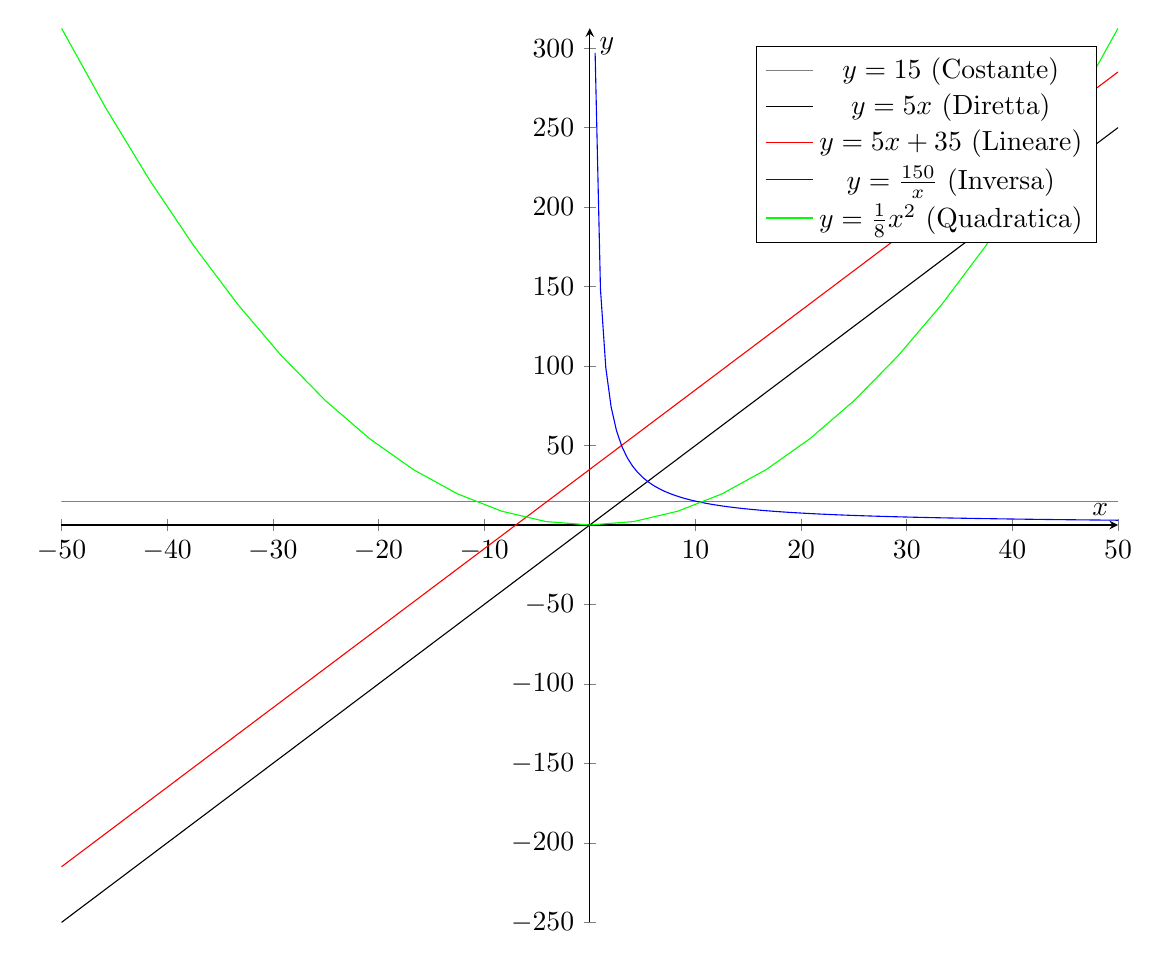
\begin{tikzpicture}
    \begin{axis}[
      axis lines = center,
      xlabel = \(x\),
      ylabel = \(y\),
    ]
      \addplot [
        domain=-50:50,
        color=gray,
      ]{15};
      \addlegendentry{\(y = 15\) (Costante)}

      \addplot [
        domain=-50:50,
        color=black,
      ]{5 * x};
      \addlegendentry{\(y = 5x\) (Diretta)}

      \addplot [
        domain=-50:50,
        color=red,
      ]{5 * x + 35};
      \addlegendentry{\(y = 5x + 35\) (Lineare)}

      \addplot [
        domain=0:50,
        color=blue,
        samples=100
      ]{150 / x};
      \addlegendentry{\(y = \frac{150}{x}\) (Inversa)}

      \addplot [
        domain=-50:50,
        color=green,
      ]{(1 / 8) * (x^2)};
      \addlegendentry{\(y = \frac{1}{8}x^2\) (Quadratica)}
    \end{axis}
    \end{tikzpicture}

    \pagebreak

    \subsubsection{Funzione Esponenziale} % Matematica - Funzioni
    La funzione esponenziale e' quella funzione definibile come

    $$ y = k^x $$

    dove l'incognita e' quindi all'esponente. Tale funzione e' definita solo per valori 
    
    $$ k \in \mathbb{R}^+ - \{1\} $$

    ovvero $ k $ strettamente maggiore di $ 0 $ e diverso da $ 1 $ \small{(Se $ k = 1 $, allora $ y = 1^x $ percio' uguale a $ 1 $, ovvero una funzione costante)}.

    \begin{tikzpicture}
    \begin{axis}[
      axis lines = center,
      xlabel = \(x\),
      ylabel = \(y\),
    ]
      \addplot [
        domain=-3:3,
        color=red,
        samples=200,
      ]{2^x};
      \addlegendentry{\(y = k^x\) con \(k > 1\)}

      \addplot [
        domain=-3:3,
        color=blue,
        samples=200
      ]{(1 / 2)^x};
      \addlegendentry{\(y = k^x\) con \(0 < k < 1\)}
    \end{axis}
    \end{tikzpicture}
  }

  Caratteristiche:
  \begin{itemize}
    \item \textbf{Asintoto}: tendenza della funzione di avvicinarsi ad un valore senza mai raggiungerlo
    \begin{quote}
      $ k > 1 $, la funzione presenta un asintoto sull'asse $ x $ per $ x $ che tende a $ -\infty $, vedi curva rossa

      $ 0 < k < 1 $, la funzione presenta un'asintoto sull'asse $ x $ per $ x $ che tende a $ +\infty $, vedi curva blu
    \end{quote}
    \item \textbf{Punti notevoli}
    \begin{quote}
      $ (0,1) $, la funzione esponenzione passa sempre per $ y = 1 $ per $ x = 0 $

      $ (1,k) $, la funzione esponenziale ha sempre valore $ k $ per $ x = 1 $
    \end{quote}
  \end{itemize}

  \pagebreak

  \subsection{Equazione Esponenziale}
  Un'equazione esponenziale e' quella che ha almeno una incognita sull'esponente. La risoluzione e' immediata usando le regole delle potenze, vedi paragrafo precedente, e riportando tutto alla stessa base.

  Esempio:

  $$ 2^{3x - 5} = 8 $$
  $$ 2^{3x - 5} = 2^3 $$

  \begin{quote}
    da qui si puo' passare al livello degli esponenti
  \end{quote}

  $$ 3x - 5 = 3 $$
  $$ 3x = 3 + 5 $$
  $$ 3x = 8 $$
  $$ x = \frac{8}{3} $$

  \subsection{Logaritmi}
  Dato il logaritmo
  $$ x = log_a(b) $$
  si dice \textbf{base} la $ a $ e \textbf{argomento} la $ b $. $ x $ e' invece un valore tale che
  $$ a^x = b $$

  Condizioni di Esistenza:
  \begin{itemize}
    \item $ a \neq 1 $
    \item $ a > 0 $
    \item $ b > 0 $
  \end{itemize}

  Proprieta':
  \begin{itemize}
    \item $ log_a(b \times c) = log_a(b) + log_a(c) $
    \item $ log_a(\frac{b}{c}) = log_a(b) - log_a(c) $
    \item $ log_a(b^c) = c \times log_a(b) $
    \item $ log_a(b) = \frac{log_c(b)}{log_c(a)} $
  \end{itemize}

  \subsection{Limiti}
  Data una funzione $ f(x) $, non definita per un suo valore $ n $, e' detto "\textit{limite di $ f(x) $ per $ x $ che tende a $ n $}" il valore cui $ f(x) $ si avvicina quando si assegna ad $ x $ un valore sempre piu' vicino ad $ n $.

  \subsubsection{Esempi} % Matematica - Limiti
  Data la funzione

  $$ y = f(x) = \frac{x^2 - 9}{x - 3} $$

  Si puo' affermare che la funzione non e' definita per $ x $ pari a 3, poiche' si avrebbe un denominatore nullo. Si puo' tuttavia stilare la seguente tabella di numeri vicini a 3:
  
  \begin{tabular}{ |c|c|c|c|c|c|c|c| }
    \hline
    \textbf{x} & 2,9 & 2,99 & 2,999 & 3 & 3,001 & 3,01 & 3,1 \\
    \textbf{y} & 5,9 & 5,99 & 5,999 & Non definita & 6,001 & 6,01 & 6,1 \\
    \hline
  \end{tabular}

  Usando la tabella, possiamo notare che i valori di $ y $ vanno avvicinandosi a 6, percio' si puo' scrivere:

  $$ \lim_{x \to 3} f(x) = 6 $$

  Similmente, data la funzione

  $$ y = f(x) = 2^x $$

  E stilando la tabella:

  \begin{tabular}{ |c|c|c|c|c| }
    \hline
    \textbf{x} & 10 & 15 & 20 & 25 \\
    \textbf{y} & 1024 & 32768 & 1048576 & 33554432 \\
    \hline
  \end{tabular}

  Possiamo notare che i valori di $ y $ aumentano a dismisura all'aumentare di x. Possiamo percio' scrivere

  $$ \lim_{x \to +\infty } f(x) = +\infty $$
\end{document}
